\documentclass[amsmath,preprintnumbers,10pt,nofootinbib,prl,twocolumn]{revtex4-1}
\usepackage{amsmath}
\usepackage{amsbsy}
\usepackage{amssymb}
\usepackage{graphicx}
\usepackage{color}
\usepackage{subfigure}
\usepackage{physics}
\usepackage{soul}
\usepackage{color}
\usepackage{bm}
\usepackage{array}
\usepackage{multirow}
\usepackage{lipsum}
\usepackage[normalem]{ulem}
%\newcommand{\Tr}{\text{Tr}}
\newcommand{\Ai}{\text{Ai}}
\newcommand{\Bi}{\text{Bi}}
\newcommand{\Real}{\text{Re}}
\newcommand{\Imag}{\text{Im}}
\usepackage{verbatim}
\usepackage{natbib}
\usepackage{nccmath}

\newcommand{\ee}{\text{e}}
\newcommand{\A}{\text{\tiny{A}}}
\newcommand{\F}{\text{ \bf F}}
\newcommand{\T}{\text{T}}
\newcommand{\U}{\text{U}}

\DeclareMathOperator\erf{erf}
\newcommand\mymathop[1]{\mathop{\operatorname{#1}}}

\def\smath#1{\text{\scalebox{0.9}{$#1$}}}
\def\sfrac#1#2{\smath{\frac{#1}{#2}}}

\newcommand\numberthis{\addtocounter{equation}{1}\tag{\theequation}}

\bibliographystyle{apsrev4-1}

\begin{document} 
\title{Structure and dissipation in active matter}
\author{ Laura Tociu$^{1,2}$*, Gregory Rassolov$^{1,2}$*, \`Etienne Fodor$^{3}$, Suriyanarayanan Vaikuntanathan$^{1,2}$}
\affiliation{$^1$The James Franck Institute, The University of Chicago, Chicago, IL,}
\affiliation{$^2$ Department of Chemistry, The University of Chicago, Chicago, IL,}
\affiliation{$^3$ DAMTP, Centre for Mathematical Sciences, University of Cambridge, Wilberforce Road, Cambridge CB3 0WA, UK}
\begin{abstract}
Structure of active matter is probed.
\end{abstract}

\maketitle



Active matter is a class of nonequilibrium systems where every component consumes energy to produce an autonomous motion~\cite{Marchetti2013, Bechinger2016, Marchetti2018}. Examples of active systems span many length- and time-scales, from bacterial swarms~\cite{Libchaber2000, Elgeti2015} and assemblies of self-propelled colloids~\cite{Bechinger2013, Palacci2013} to animal groups~\cite{Cavagna2010, Cavagna2014} and human crowds~\cite{Bottinelli2016, Bartolo2019}. The energy fluxes stemming from individual self-propulsion lead to complex collective behaviors without any equilibrium equivalent, such as a collective directed motion~\cite{Dauchot2010, Sood2014} and phase separation despite purely repulsive interactions~\cite{Bechinger2013, Palacci2013}. The possibility of exploiting such behaviors to design materials with innovative functions is a motivation for learning how to reliably predict and control the features of active systems.


Minimal models have been proposed to capture active dynamics, for instance with either aligning or isotropic particles, yielding respectively collective motion~\cite{Vicsek1995, Chate2020} and motility-induced phase separation (MIPS)~\cite{Fily2012, Cates2015}. Based on these models, the challenge is to establish a nonequilibrium thermodynamic framework, by analogy with equilibrium, which connects microscopic details and emergent physics. Progress has been made in this direction by characterizing protocol-based observables, such as pressure~\cite{Marchetti2014, Brady2014, Solon2015}, surface tension~\cite{Speck2015, Paliwal2017, Zakine2020}, and chemical potential~\cite{Paliwal2018, Guioth2019}. Importantly, the dissipation induced by microscopic energy fluxes has recently attracted much attention, since it measures the cost to drive the dynamics into nonequilibrium states~\cite{Shim2016, Suma2017, Junco2018, Spinney2018, Murrell2018, Murrell2019, Markovich2020} and to extract work with original protocols~\cite{Zakine2017, Martin2018, Pietzonka2019, Liao2020, Ekeh2020, Kroy2020}. In particular, it has been shown that dissipation constrains the transport of active particles~\cite{Suri2019, Suri2020}, and that changing dissipation with a dynamical bias yields changes in material properties~\cite{Suri2019} and some phase transitions~\cite{Nemoto2019, Suri2020,GrandPre2020}. The dissipation rate can also be connected to the mechanical properties, such as the so called active pressure, of certain isotropic active matter models. 

Evaluating the dissipation, however, requires microscopic information which can be difficult to access. Indeed, in the context of the commonly used active matter models, information about the polarization or self-propulsion of an active particle is required to compute the dissipation rate. Such information might be tough to access in experiments. Indirect measurements have then been proposed, which rely either on estimating the response to perturbation~\cite{Sasa2005, Toyabe2010, Ahmed2016, Nardini2017, Mizuno2018}, quantifying currents~\cite{Barato2015, Gingrich2016, Gladrow2016, Li2019}, or analyzing the irreversibility of trajectories~\cite{Roldan2018, Parrondo2019}. However, such measurements re still very data intensive[Something along these lines to motivate our work]. 

Interestingly, and of particular relevance to this current work, some of us have recently revealed an empirical relation between dissipation and microscopic structure which alleviates many of the limitations of indirect measurements~\cite{Suri2019}. While this result potentially encompasses a broad scope of applications, since it allows for extracting energy current from measurements of density pair correlations only, any systematic derivation has remained elusive. Moreover, its applicability close to phase transitions is also  largely an open question.

In this paper, we develop a non-equilibrium mean field theory that elucidates connections between the microscopic structure and dissipation rate in a model class of active matter system. Our central results analytically verify the empirical connection in ~\cite{Suri2019} and show how it might be possible to infer the dissipation simply from static two body configurational correlations in a broad range of regimes. Unlike existing approaches, our result does not need any trajectory information or information related to experimentally tough to access polarization data. Further, at variance with existing approaches that mainly work in weakly interacting regimes~\cite{Dean_1996}, our analytical mean field theory works surprisingly well in systems with strong interactions. Further, unlike other effective representations of active dynamics~\cite{Maggi2015, Rein2016, Wittmann2017}, we do not rely on any equilibrium approximation, thus allowing one to retain all nonequilibrium features, and in particular to evaluate properly the dissipation.

Finally, motivated by this set of results, we show that it is in fact possible to construct a machine learning setup that can infer the dissipation rate just from just the static structure of an active fluid. This result opens the door for the design of adaptive strategies in which the dissipation rate is adjusted till a desired non-equilibrium structure or pattern is obtained. 

The rest of the paper is organized as follows. First, we describe the model active matter system used in this paper. Next, we describe our novel non-equilibrium mean field theory and show how it helps anticipate the structure of a fluid surprisingly well even in cases with strong interactions. This non-equilibrium mean field theory is then used to analytically show a connection between the static two body positional correlations and the dissipation rate of the active media (need to clarify that the connection is in some regimes). This connection is verified using extensive simulations. Finally, we show how a machine learning setup can infer the overall dissipation rate from just static positional snapshots of the active liquid. Together, our analytical and numerical results show how dissipation can be used to productively engineer the structure of active matter systems. 


%In this paper, (1) we develop a nonequilibrium mean-field theory which accurately describes the dissipation and structure of an assembly of active particles. Inspired by previous works~\cite{Demery2011, Demery2014}, our approach relies on deriving the effective dynamics of an active tracer embedded in the system. At variance with other effective representations of active dynamics~\cite{Maggi2015, Rein2016, Wittmann2017}, we do not rely on any equilibrium approximation, thus allowing one to retain all nonequilibri

%(2) Further, we illustrate the utility of our theory by showing how it can be applied to even strongly driven systems. This is achieved by replacing -v(k)/T with c(k), motivated by traditional equilibrium liquid state theories. (3) Based in part on this mean field theory, show how $\dot{w}  \propto \cal{I}$ (Gaussian approximation is used additionally). (4) Verify connections in (3) for WCA particles.  (5) Use machine learning to show dissipation can be inferred from static structure, which confirms (3) from a different perspective.


%strongly driven systems approaching a non-equilibrium phase transition.

%In this paper we work out [Outline] (1) A mean field theory for the structure of an active liquid (2) Show how the mean field theory works fairly well even for strongly driven systems. This is done using c(k) instead of -v(k). (3) Based in part on this mean field theory, show how $\dot{w}  \propto \cal{I}$ (Gaussian approximation is used additionally). (4) Verify connections in (3) for WCA particles.


% We consider a popular model of active matter made of interacting self-propelled particles, often referred to as Active Ornstein Uhlenbeck Particles (AOUPs)~\cite{Szamel2014, Maggi2015, Nardini2016}, with two-dimensional overdamped dynamics:
% \begin{equation}
%	\dot{\bf r}_i = -\mu\nabla_i \sum_{j\neq i} u({\bf r}_i-{\bf r}_j) + {\bf v}_i + {\boldsymbol\xi}_i ,
%\end{equation}
% where $\mu$ is the mobility, and $u$ is the pair-wise potential. The terms $\{{\boldsymbol\xi}_i,{\bf v}_i\}$ embody respectively the thermal noise and the self-propulsion velocity. They have Gaussian statistics with zero mean and uncorrelated variances, given by $\langle\xi_{i\alpha}(t)\xi_{j\beta}(0)\rangle = 2D \delta_{ij}\delta_{\alpha\beta}\delta(t)$ and $\langle v_{i\alpha}(t)v_{j\beta}(0)\rangle = (D_{\rm A}/\tau) \delta_{ij}\delta_{\alpha\beta}e^{-|t|/\tau}$, where $\{D,D_{\rm A}\}$ are respectively the passive and active diffusion coefficients, and $\tau$ is the persistence time. For a vanishing persistence ($\tau=0$), the system reduces to a set of passive Brownian particles at temperature $(D+D_{\rm A})/\mu$. At sufficiently high persistence, the system undergoes a phase separation even with purely repulsive interactions~\cite{Nardini2016, Maggi2020}.



 

\section{A non-equilibrium mean field theory for the structure and dissipation of an active fluid}.

We consider a popular model of active matter made of interacting self-propelled particles, often referred to as Active Ornstein Uhlenbeck Particles (AOUPs)~\cite{Szamel2014, Maggi2015, Nardini2016}, with two-dimensional overdamped dynamics:
 \begin{equation}
	\dot{\bf r}_i = -\nabla_i \sum_{j\neq i} u({\bf r}_i-{\bf r}_j) + {\bf v}_i + {\boldsymbol\xi}_i ,
\end{equation}
 where $u$ is the pair-wise potential and units have been chosen to ensure a unit mobility. The terms $\{{\boldsymbol\xi}_i,{\bf v}_i\}$ embody respectively the thermal noise and the self-propulsion velocity. They have Gaussian statistics with zero mean and uncorrelated variances, given by $\langle\xi_{i\alpha}(t)\xi_{j\beta}(0)\rangle = 2T \delta_{ij}\delta_{\alpha\beta}\delta(t)$ and $\langle v_{i\alpha}(t)v_{j\beta}(0)\rangle = (T_{\rm A}/\tau) \delta_{ij}\delta_{\alpha\beta}e^{-|t|/\tau}$, where $\tau$ is the persistence time. For a vanishing persistence ($\tau=0$), the system reduces to a set of passive Brownian particles at temperature $T+T_{\rm A}$. At sufficiently high persistence, the system undergoes a phase separation even with purely repulsive interactions~\cite{Nardini2016, Maggi2020}. 


%We consider an overdamped active matter system in 2D consisting of spherical particles interacting through a pairwise potential $\U = \sum_i \sum_{j\neq i} u(r_{ij})$ and subject to white noise ${\bm \xi}$ and a self-propulsion force ${\bf f}$ as follows:
%\begin{equation}\label{eq:dyn}
%\dot{\bf r}_i = \dfrac{{\bf f}_i - \nabla_i \U}{\gamma} + {\bm \xi}_i ,
%\end{equation}
%where $\gamma$ is the damping coefficient. In all subsequent %calculations, $\gamma$ is set to 1 so it is not explicitly included in derivations anymore. The white noise mimics fluctuations from the thermal the bath and has correlations:
%\begin{equation}
%\langle \xi_{i\alpha}(t) \xi_{j\beta}(0) \rangle = \dfrac{2 \T }{\gamma} %\delta_{ij} \delta_{\alpha\beta} \delta(t) ,
%\end{equation}
%where the $ij$ and $\alpha\beta$ indices refer to particle labels and spatial components, respectively. The Boltzmann constant $\text{K}_{\text{B}}$ is set to 1, so that in the absence of self-propulsion and particle interactions, the fluctuation dissipation relation $\text{D} = \tfrac{\text{K}_{\text{B}} \T}{\gamma}$ is obeyed. 

%The particles we consider are known as Active Ornstein-Uhlenbeck particles (AOUP). 
%The  self-propulsion forces are modelled as Ornstein-Uhlenbeck processes:
%\begin{equation}\label{eq:v}
%\tau\dot{\bf f}_i=-{\bf f}_i+{\bm \eta}_i ,
%\end{equation}
%where ${\bm \eta}_i$ is a zero-mean Gaussian white noise, uncorrelated with ${\bm %\xi}_i$, with correlations:
%\begin{equation}\label{eq:noise}
%\langle\eta_{i\alpha}(t)\eta_{j\beta}(0) \rangle = %2\T_{\A}\delta_{ij}\delta_{\alpha\beta}\delta(t)
%\end{equation}
% This next paragraph is copied from NJP.
%For a vanishing persistence time $\tau$, the active fluctuations cannot be distinguished from
%the thermal ones: $\langle f_{i\alpha}(t) f_{j\beta}(0) \rangle = 2 \T_{\A} \delta_{ij} \delta_{\alpha\beta} \delta(t)$, in which case the system amounts to a set of passive %Brownian particles at temperature $\T + \T_{\text{\tiny A}}$. 

%The correlations of the self-propulsion forces are:
%\begin{equation}\label{eq:active_corr}
%\langle f_{i\alpha}(t) f_{j\beta}(0) \rangle = \frac{\T_{\A}}{\tau} \delta_{ij} %\delta_{\alpha\beta} e^{-|t|/\tau}
%\end{equation}
%where $\T_{\A}$ sets the strength of the self-propulsion.

To make analytical progress on this model, we begin by considering the effective dynamics of an active tracer embedded in a bath consisting of the other particles. As in recent work (\cite{Demery2011, Demery2014}), we scale the interaction strength between the tracer and the bath by a dimensionless parameter $h$. The equation of motion of the tracer ${\bf r}_0(t)$ reads:

\begin{equation}\label{eq:dyn_pert}
\dot{\bf r}_0 = {\bf f}_i - h \int  \nabla \U({\bf r}  - {\bf r}') \rho ({\bf r}', t)  d {\bf r}' + {\bm \xi}_i ,
\end{equation}
where the bath is described in terms of the density field $\rho ( {\bf r} , t) = \sum_i \delta({\bf r} - {\bf r}_i(t))$ and $i$ indexes the bath particles. When $h=0$, the tracer is not coupled to the bath, while when $h=1$ the tracer is fully coupled to the bath.

An equation of motion for the density field, $\rho({\bf r} , t)$, can be readily obtained following the procedure in Ref~\cite{Dean_1996} with an added polarization term $ \F ({\bf r}, t) = \sum_i {\bf f}_i \delta({\bf r} - {\bf r}_i(t))$ that comes from the activity:
\begin{align*}\label{eq:field_EOM}
    \dfrac{\partial \rho ({\bf r}, t)}{ \partial t} & = \nabla \cdot \left( \rho \nabla \left[ \int  \U({\bf r}  - {\bf r}') \rho({\bf r}', t)  d {\bf r}' +  h\U({\bf r} - {\bf r}_0)  \right] \right) \\
    & + \T \nabla^2 \rho({\bf r}, t) + \sqrt{2 \rho \T} {\bm \Lambda}({\bf r}, t) -\F({\bf r}, t) ), \numberthis
\end{align*}
where we include the effect of the tracer on the bath dynamics through the term scaled by $h$. The last term is a multiplicative noise that acts as a fluctuating force:
\begin{equation}\label{eq:field_noise}
     \langle {\bm \Lambda}_{\alpha} ({\bf r}, t) {\bm \Lambda}_{\beta} ({\bf r}', t') \rangle = \delta_{\alpha \beta} \delta({\bf r} - {\bf r}') \delta(t - t') 
\end{equation}


%Deriving equations for the structure of the liquid and the dissipation rate requires a solution for the density field first, followed by an expansion in the parameter $h$. 
In principle, Eq.~\ref{eq:dyn_pert} and Eq.~\ref{eq:field_EOM} can be solved recursively to obtain estimates of the density field $\rho({\bf r} , t)$. This estimate can in turn be used to compute the two body pair correlation function, $g({\bf r} )$
\begin{equation}\label{eq:gk}
\rho_0 g({\bf k}) = \left \langle  e^{i{\bf k} \cdot {\bf r}_0 (t) } \rho ({\bf k}, t) \right \rangle,
\end{equation}. 
%The averaging is understood to be performed over the white noise in Eq. \ref{eq:noise}, the  multiplicative noise in Eq. \ref{eq:field_noise_k} and at a single time point once the system has settled in its non-equilibrium steady-state.

Similarly, we can also use this setup to obtain expressions for "rate of work", which denotes the change in the energy of the system due to the action of non-conservative forces~\cite{Suri2019,Suri2020,delJunco_2018}, by computing:
\begin{equation}\label{eq:wdot}
    \dot{w} = \langle {\bf f}_i \cdot \nabla_i U  \rangle = h \left \langle {\bf f}_i(t) \cdot i{\bf k} \U({\bf k}) \delta \rho({\bf k}, t) \right \rangle,
\end{equation}
This rate of work, $\dot{w}$, is a quantification of the energy dissipation in the system~\cite{Suri2019}. In practice, due to the non-linear nature of the equations, exact solutions for the density field $\rho({\bf r} , t)$ can be rarely obtained. For weakly interacting systems, expressions for $\rho({\bf r} , t)$ can be obtained perturbatively. In this regime, analytical expressions for $\dot{w}$ and $g({\bf r} )$ can then be derived. However, such results cannot be readily extended to strongly interacting systems. Hence, to the best of our knowledge, there is very little analytical work characterizing non-equilibrium structure and dissipation in far from equilibrium strongly interacting systems. 

Here, we attempt to take the first steps towards such a framework by building a mean field theory. The central element of our approach is insight obtained from the study of simple strongly interacting liquids that suggests that the so called directed correlation function, $c(r)$, provides a more natural basis to organize a perturbation theory. Indeed, at equilibrium, the effect of adding a weak perturbation $w(r)$ to a strong interparticle potential can be readily accounted for using the relation $c_{\rm eq}^{\rm perturb}(r) \approx c_{\rm eq}(r) + w(r)$, where $c_{rm eq}(r)$ is the direct correlation function of the original fluid and $c_{\rm eq}^{\rm perturb}(r)$ is the new direct correlation function. Since the direct correlation function and two body correlation function are connected by the Ornstein-Zernike relation, the two body correlation function of the perturbed fluid can now be accessed. Further, in the context of equilibrium solvation theories, it has been shown that the effect of introducing a tagged solvent molecule into a bath of solvent molecules can be accounted for by considering a convolution of the direct correlation function with the density field of the solvent. For weakly interacting systems, the direct correlation function is simply proportional to the pair-wise interactions , $-k_B T c_{\rm eq}(r)=U(r)$ and the standard linear response theory is recovered. 

Motivated by these findings, we write down a mean field theoretical framework for our system by replacing $U(k)$ in Eq.~\ref{eq:dyn_pert} and Eq.~\ref{eq:field_EOM} with $-k_B T c_{\rm eq}(k)$, where $c_{\rm eq}(k)$ is the Fourier transform of the equilibrium direct correlation function of our fluid. As described in the SI Section I, we construct a perturbation expansion in the coupling parameter $h$ to compute the two body correlation function. The first term in the expansion leads to the following expression: 
\begin{align*}\label{eq:final_expression_gr}
g({\bf k}) = &
 -  |{\bf k}|^2 (-c_{\rm eq}({\bf k}))  \dfrac{ G({\bf k}) + \T}{G({\bf k})} \cross \\
& \int
_{-\infty}^0 ds e^{|{\bf k}|^2 ( G({\bf k}) + \T)s}  e^{-|{\bf k}|^2 R(-s)/2}\numberthis
\end{align*}
where 
\begin{equation*}
R(s) = 2\T_\A s - 2 \T_\A \tau (1 - e^{-s/\tau}) 
\end{equation*}
where $G({\bf k}) \equiv \rho_0 -c_{\rm eq}({\bf k}) + T$, $g({\bf k})$ dentoes the Fourier transform of the two body pair correlation function $g(r)$. In the equilibrium limit of no activity, we recover the standard Ornstein-Zernike relation from Eq.~\ref{eq:final_expression_gr}. 
As explained in the SI Section I, the perturbation theory leading up to the expression in Eq.~\ref{eq:final_expression_gr} also ignores the effect of activity terms in Eq.~\ref{eq:field_EOM}. Previous work by some of us where we obtained expression for $\dot{w}$ in a weakly interacting system using a path-integral approach~\cite{Suri2020}, noted that numerical contribution from such terms is negligible. 

In Fig.~\ref{Fig:1}, we plot the Fourier transform of the predicted non-equilibrium direct correlation function, $c({\bf k})\equiv g({\bf k})/(1+\rho g({\bf k}))$ from theory (Eq.~\ref{eq:final_expression_gr}) along with estimates obtained from simulations. The only input for this theory is the equilibrium direct correlation function. The simulations were performed at $T_A=30$ and $\tau=0.4$ with a density of $\rho=1$. We used a short ranged interparticle potential $U({\bf r})=A (1- r)^2, r\leq 1$ with $A=16 k_b T$. Our theory does a surprising good job of predicting the non-equilibrium direct correlation function, in particular the long wavelength parts. We also note that our approach is not perfect and that there are discrepancies in the high wavenumber regimes indicating that our approach doesn't completely capture all the packing effects due to non-equilibrium activity. However, our mean field approach still performs dramatically better than the the existing techniques which are valid mainly in the weak interaction limit fail in the strongly interacted regimes regime~\cite{Dean_1996,Demery2011}. We now use this mean field theory to study connections between the structure and dissipation of non-equilibrium fluids. 
\begin{figure}
    \centering
    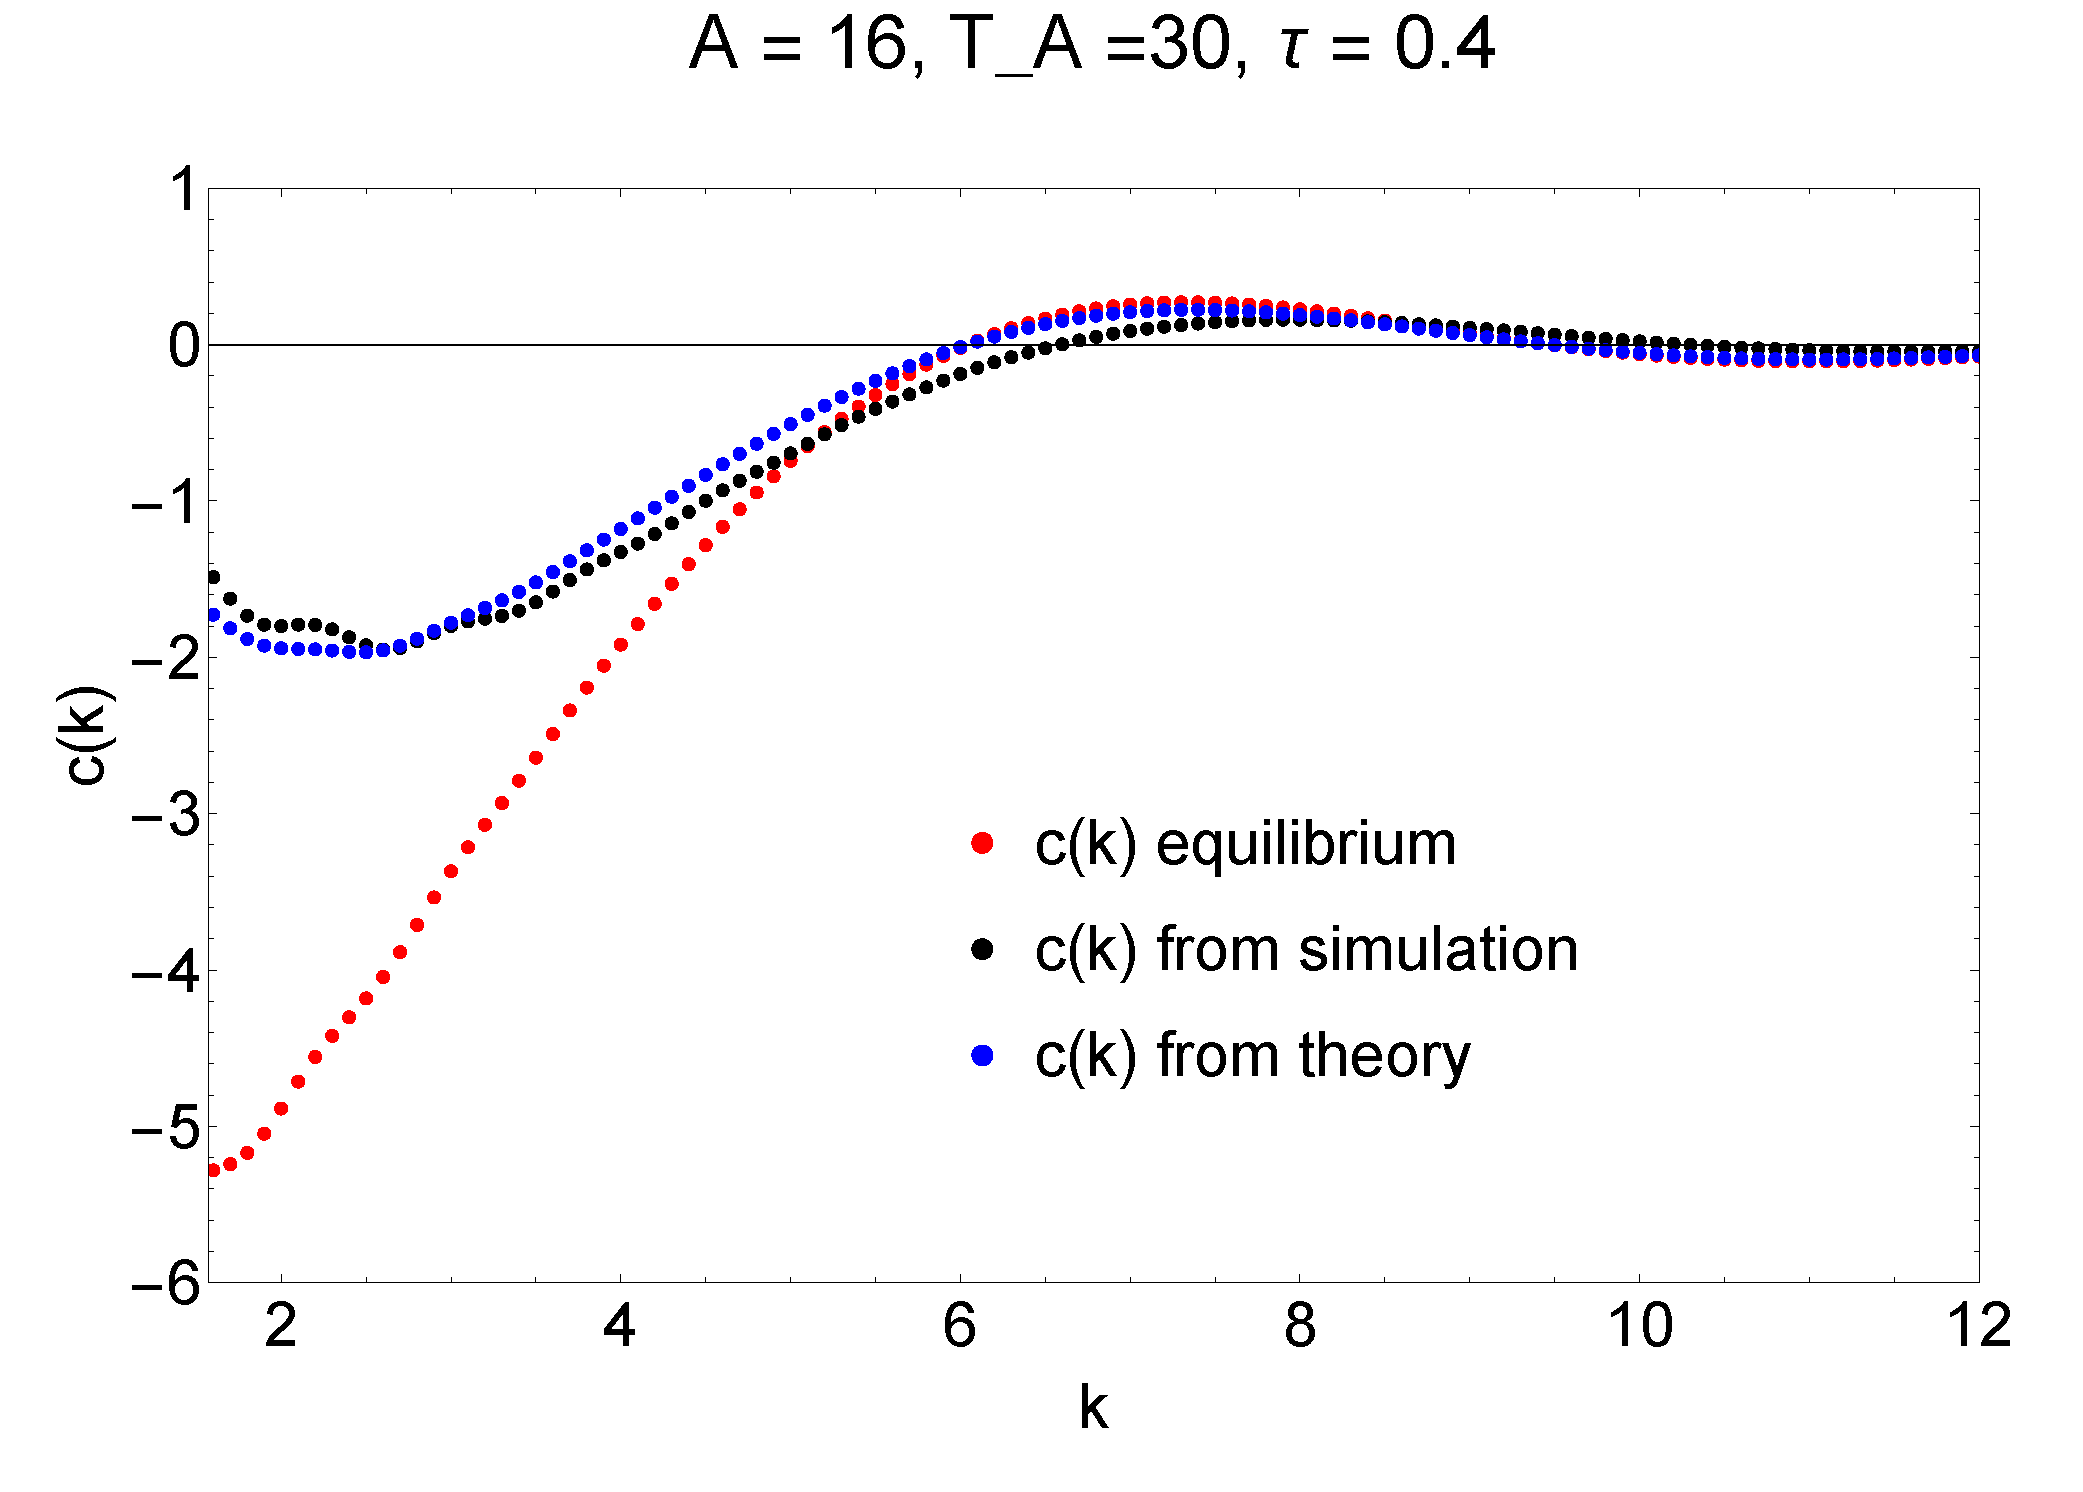
\includegraphics[scale=0.25, clip=True]{Ck_A16_T30_U0.4.pdf}
    \caption{Prediction for c(k) in a strongly driven system of harmonic disk particles (blue), compared with predicted c(k) for the system with no driving (red) and measured c(k) from simulation with driving (black). $\rho = 1.00, A = 16, \tau = 0.4, T_A = 30$ (blue, black); $T_A = 0$ (red).}
    \label{Fig:1}
\end{figure}

\section{Connection between dissipation and structure}
We begin by following the mean field construction described in the previous section and set up a perturbation theory to evaluate the expression for rate of work. The first term in this expansion leads to the following expression for the rate of work. 
\begin{align*}\label{eq:final_expression_wdot}
    \dot{w} & = h^2 \rho_0 \dfrac{T_\A}{\gamma^2} \int d{\bf k} |{\bf k}|^4 (U({\bf k}))^2 \dfrac{ G({\bf k}) + T/ \gamma}{G({\bf k})} \cross \\
& \int_{-\infty}^0 ds e^{|{\bf k}|^2 ( G({\bf k}) + T/ \gamma)s}  e^{-\frac{|{\bf k}|^2}{\gamma^2} R(-s)/2} (1-e^{s/\tau}) \numberthis
\end{align*}



In Ref.~\cite{Suri2019} some of us empirically noted that the rate of work, $\dot{w}$ can be connected to the two body density correlation function, $g(\bf r)$, through the relation
\begin{equation}
    \dot{w}=\alpha (\tau) \int \left[\nabla U({\bf r})^2)-\nabla^2 U({\bf r})\right][g({\bf r})-g_{\rm eq}({\bf r})]\equiv \alpha (\tau) \tilde I
\end{equation}
where the factor $\alpha(\tau)$ is a function of the interaction potential, density, and $\tau$ but is crucially independent of $Pe\equiv \sqrt{Ta/\tau}$. This empirical connection was noted for a WCA fluid and allowed for the exciting possibility that the dissipation rate of an active fluid can be inferred just from the static structure. Our mean field theory allows us to provide an analytical justification for this connection. 

Indeed, in Fig.~\ref{fig:2} we plot estimates of $\dot{w}$ and $\tilde I$ obtained from simulations and from our analytical theory. The simulations were performed with the While the exact values of $\dot{w}$ and $\tilde I$ predicted are off when compared to the simulation values \texendash this is consistent with above noted deviation in the short length scale structure predicted by our theory \texendash, our theory performs surprising well in predicting 

%The results obtained so far are in the low-activity and weak-potential limit. However, setting $h=1$ in our final, perturbation theory results for $g({\bf k})$ and $\dot{w}$ an yields excellent agreement with simulation data for strong driving. // This suggests the terms we neglected (higher order terms in the perturbation theory, as well as the polarization in the field EOM) are small or cancel. // -- needs rephrasing and more thought.

%Coupled with our novel substitution described in the next section, the mathematical trick of setting $h=1$ further allows us to predict dissipation and structure at arbitrary activity and interaction strength with reasonable accuracy.

\begin{figure}
    \centering
    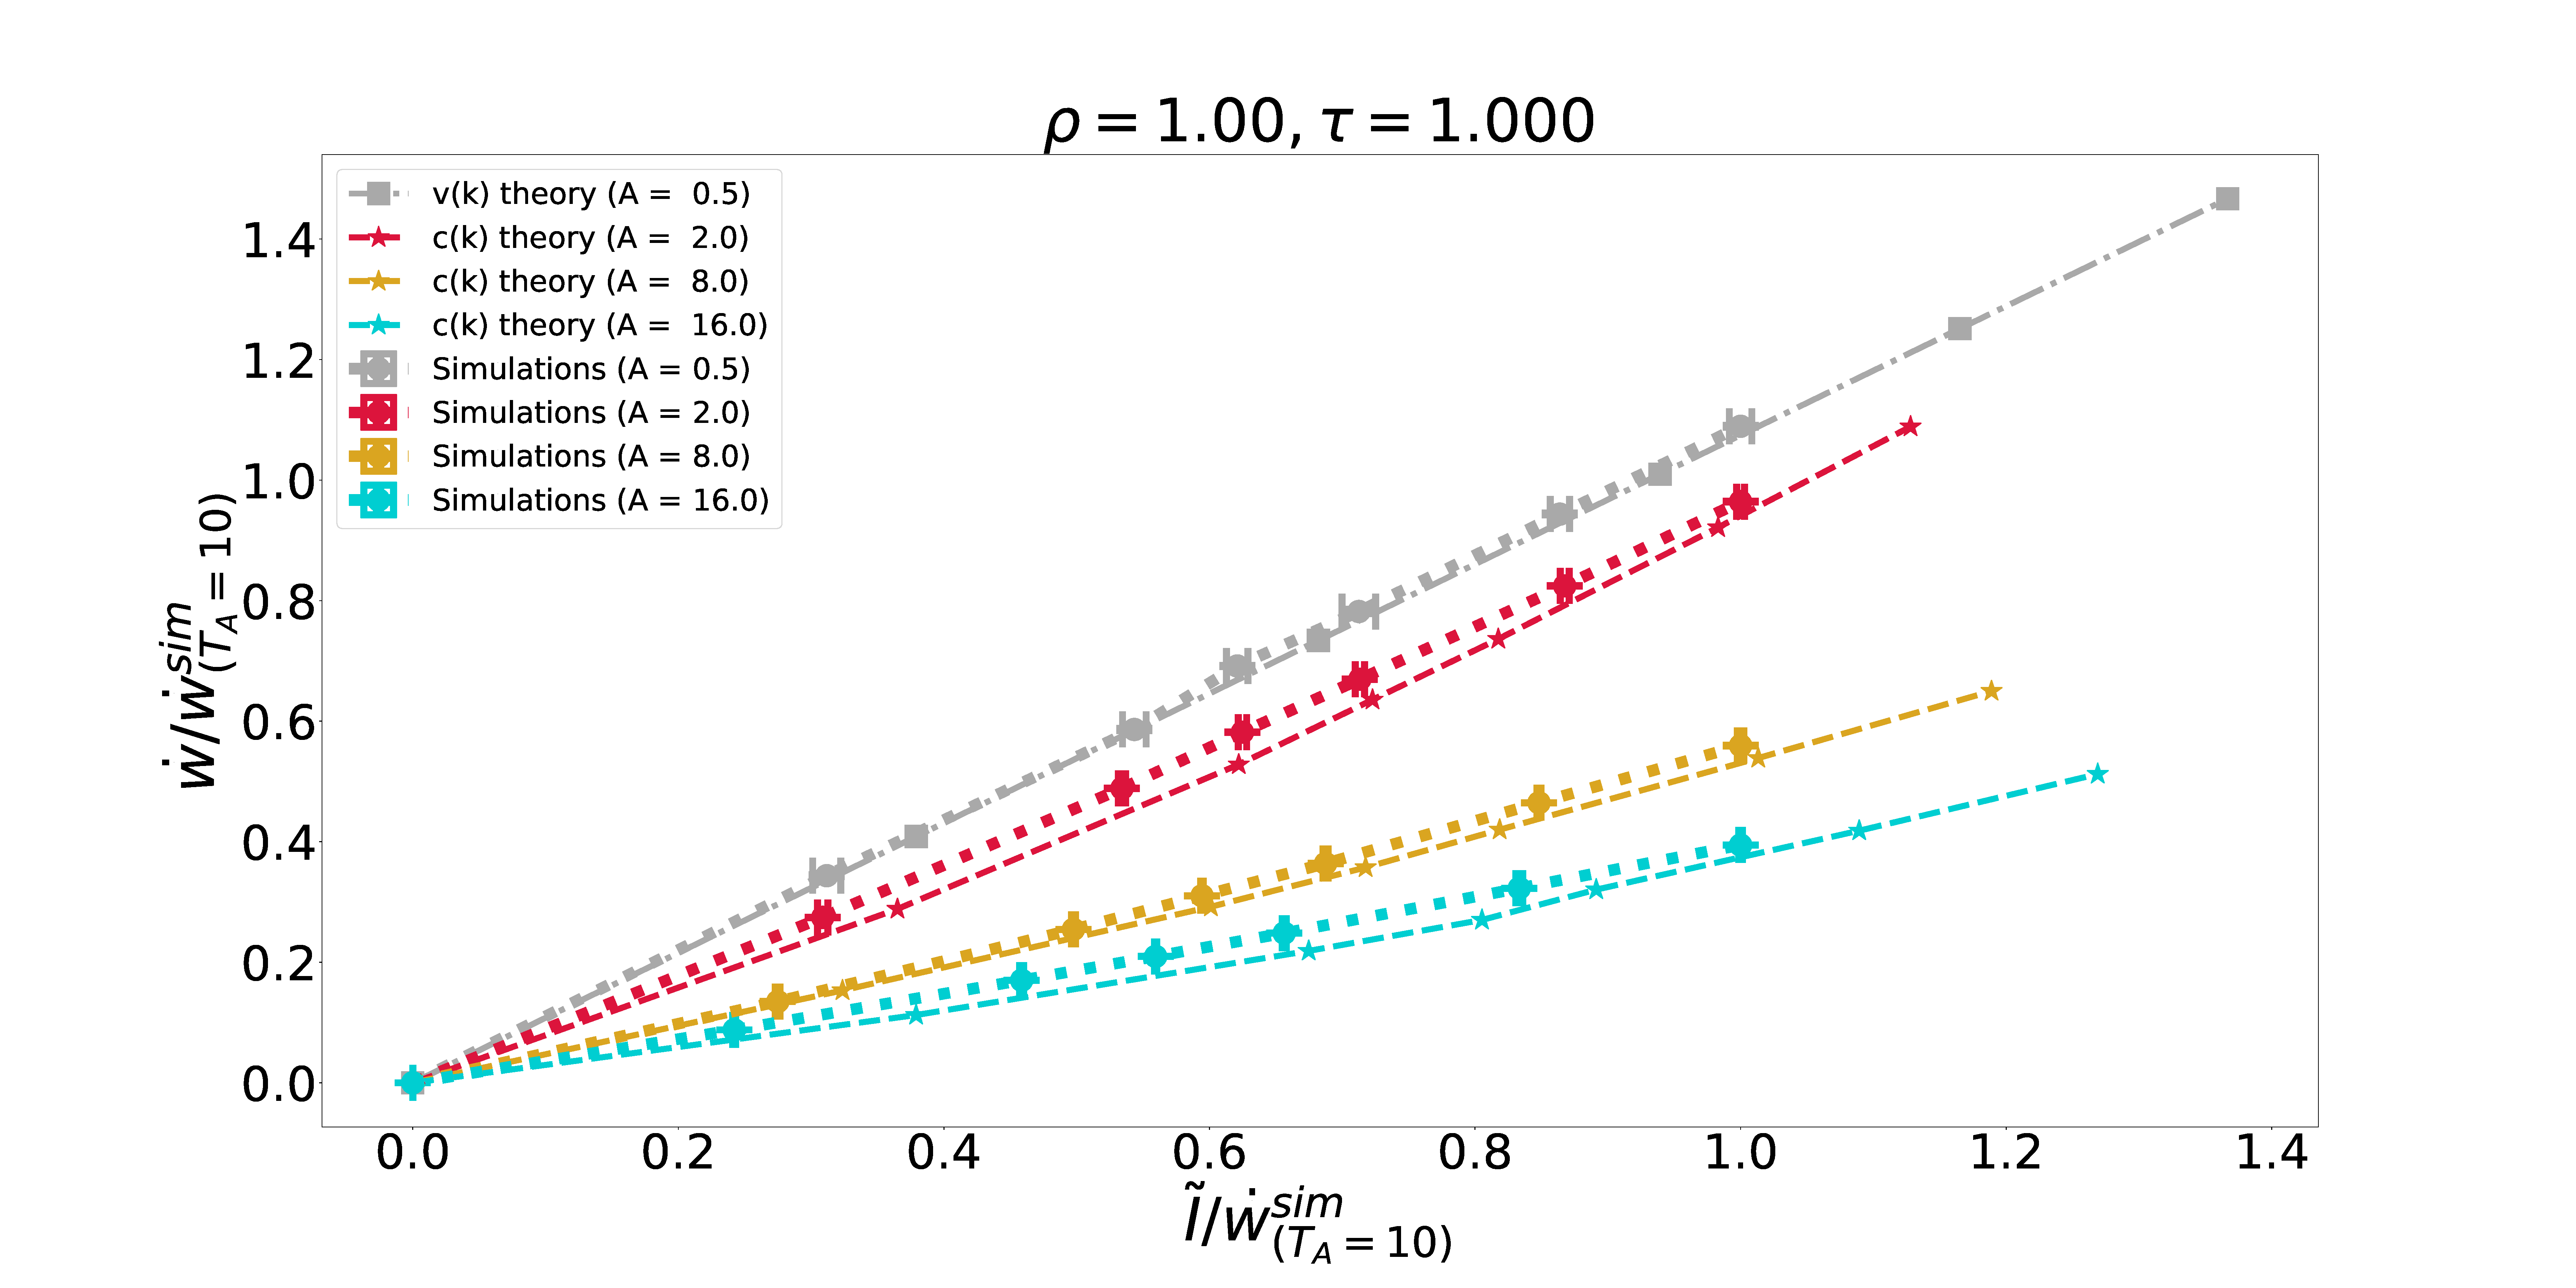
\includegraphics[scale=0.075, clip=True]{dW_tI_new_Suri_R1.00_U1.000.pdf}
    \caption{Prediction for c(k) in a strongly driven system of harmonic disk particles (blue), compared with predicted c(k) for the system with no driving (red) and measured c(k) from simulation with driving (black). $\rho = 1.00, A = 16, \tau = 0.4, T_A = 30$ (blue, black); $T_A = 0$ (red).}
    \label{Fig:2}
\end{figure}

-----SURI IS HERE--------
\section{C(k) Substitution}
We begin by neglecting the polarization term, which amounts to considering a passive bath. Our choice is justified in the low-activity limit and supported by the results in \cite{Suri2020}. // In this work, the formulas for efficiency and mobility (Appendix equations A.8 and A.9) were obtained by setting two-point polarization correlators to zero. The results agree with simulation data very well at strong driving, too. // -- needs rephrasing and more thought. The resulting closed-form equation of motion can be linearized around the density $\rho_0$ of the particles by writing $\rho ({\bf r}, t) = \rho_0 + \delta \rho({\bf r}, t)$ and discarding the terms quadratic in $\delta \rho$. This approximation holds for weak interparticle potentials so that any local density fluctuation is small compared to the density of the liquid. 

After linerization, the solution for $\delta \rho({\bf k}, t) = \int [ \rho({\bf r}, t) - \rho_0) ] e^{-i{\bf k} \cdot {\bf r}} d{\bf r}$ follows readily as:

\begin{align*}\label{eq:red_field_EOM_k}
\delta \rho( {\bf k}, t) & = \int_{-\infty}^t e^{-|{\bf k}|^2 G({\bf k}) (t-s)} \left( -h |{\bf k}|^2 \rho_0 \U({\bf k}) e^{-i{\bf k} \cdot {\bf r}_0(t - s)} \right. \\
& \left. + i{\bf k} \cdot \sqrt{2\rho_0 \T} \bm{\Lambda} ({\bf k}, s) \right),\numberthis
\end{align*}
where $G({\bf k}) = \rho_0 \U({\bf k}) + \T$ and $\bm{\Lambda}$ is a multiplicative noise term obeying:
\begin{equation}\label{eq:field_noise_k}
\langle {\bm \Lambda}_{\alpha}({\bf k}, s)  {\bm \Lambda}_{\beta}({\bf k}', s')  \rangle = \delta_{\alpha \beta}\delta(s-s')\delta({\bf k} + {\bf k}')
\end{equation}


To be filled out

\section{$\mathcal{I}$ versus $\dot{w}$}

To be filled out

\section{Machine Learning}

Our goal in this section is to use a machine learning infrastructure most closely related to a convolutional neural network to map snapshots of AOUP particles to the energy dissipation encoded in them. 

To this extent, we designed a network consisting of a continuous convolutional layer followed by a dense layer (Fig. \ref{Fig:ML}). The continuous convolutional layer is inspired by recent work on rotationally and translationally invariant networks for atomic systems \cite{tess2018}. 

- From here on out it should be in the SI, I think -
The network was built in keras using the Functional API \cite{keras}. The individual input to the network consists of an array of size $N \cross D$ that contains, for each of the N particles, the distances to its nearest $D$ neighbors. For the simulations with the harmonic potential, $N = 625$ and $D = 25$, while for the simulations with the Yukawa potential, $N = 312$ and $D = 20$. The choice of $D$ was such that distances to around $r = 3$ (even $r = 4$) are mostly captured, but with certainty all distances up to the cutoff ($r = 1$ for harmonic and $r=2$ for Yukawa) are captured. Such a choice ensures that the algorithm has access to all the distances that we expect are crucial to extracting the rate of work, but also simplifies the implementation by allowing a rectangular input shape.

The continuous convolutional layer is built as a custom layer and performs the following:
For each convolution center, in this case an AOUP particle ${\bf r}_i$, the convolution operation consists of evaluating the sum $\sum_{j=1}^{D} F({\bf r}_{ij})$. Here, $F$ is a learnable function, the equivalent of a filter in traditional convolutional neural networks.  Inspired by our connection between interparticle distances and rate of work in Section XXX (Eq. YYY), we relax the function $F$ to be a radial function, and we express it in a basis of $N_G=16$ Gaussian functions centered between $r=0$ and $r=3$ and with a standard deviation of 0.1:

\begin{equation}
    F(r) = \sum_{i=0}^{15} \beta_i e^{-(r-0.2 i)^2/(2\cdot 0.1)^2}
\end{equation}

In the dense layer, we enforce particle indistinguishibility by setting a constraint that the weights $u_i = u $ are identical. 

Finally, the output to the network consists of the rate of work $\dot{w}$, centered as:

\begin{equation}
    \dot{w}_{\text{centered}} = \dot{w} + \alpha \int 2\pi r (\nabla u(r)^2 - \nabla^2 u(r)) g_{eq}(r) dr
\end{equation}

and rescaled as:

\begin{equation}
    \dot{w}_{\text{rescaled}} = \dfrac{\dot{w}_{\text{centered}}}{\max(\dot{w}_{\text{centered}}) - \min(\dot{w}_{\text{centered}} )}
\end{equation}

The rate of work is calculated at each value of $T_A$ as detailed in the main text. Multiple individual snapshots at the same value of $T_A$ will have the same output.

In conclusion, the machine performs the following mapping from the interparticle distances $r_{ij}$ to the output (rescaled rate of work):

\begin{equation}
     u \sum_i \sum_{j} \sum_{k=0}^{15} \beta_k e^{-(r_{ij}-0.2 i)^2/(2\cdot 0.1)^2} + b = \dot{w}_{\text{rescaled}}
\end{equation}

The machine is tasked with finding the best $u, \beta_k$ and $b$ to minimize the deviation between its predicted output $\dot{w}_{\text{pred}}$ and $\dot{w}_{\text{rescaled}}$. We choose to quantify this deviation through a loss function of the form:

\begin{equation}
     L(\{\dot{w}^a_{pred, i}\}) = \sum_a 1/N_a \sum_i (\dot{w}^a_{pred, i} - \dot{w}_{\text{rescaled}})^2,
\end{equation}
where the $a$ indexes the $T_A$ values used in the training process.  Our choice of loss function ensures that the rate

Acknowledging that in the large $N$ limit, $ \int 2\pi r F(r) g(r) dr = 1/N \sum_i \sum_j F(r_{ij})$, and using Eq. YYY, it follows that the machine learning could, in principle, learn the mapping exactly by setting $b = 0$, $ u = \alpha/(\text{N} (\max(\dot{w}_{\text{centered}}) - \min(\dot{w}_{\text{centered}} ))$ and learning the function $F(r)$ as $\nabla u(r)^2 - \nabla^2 u(r)$.

- Now back to the main text - 

We prepared 6000 snapshots for harmonic and 3000 snapshots for Yukawa, and divided them into train/validation/test (0.7/0.15/0.15). We ran 5 trials until we observed convergence of the validation loss (between 100 and 300 epochs of training), using the adam algorithm in keras with batch size 512. In Figures 12 and 13 we show the agreement between the real and predicted $\dot{w}$, averaged over 5 trials. 


\begin{figure}
    \centering
    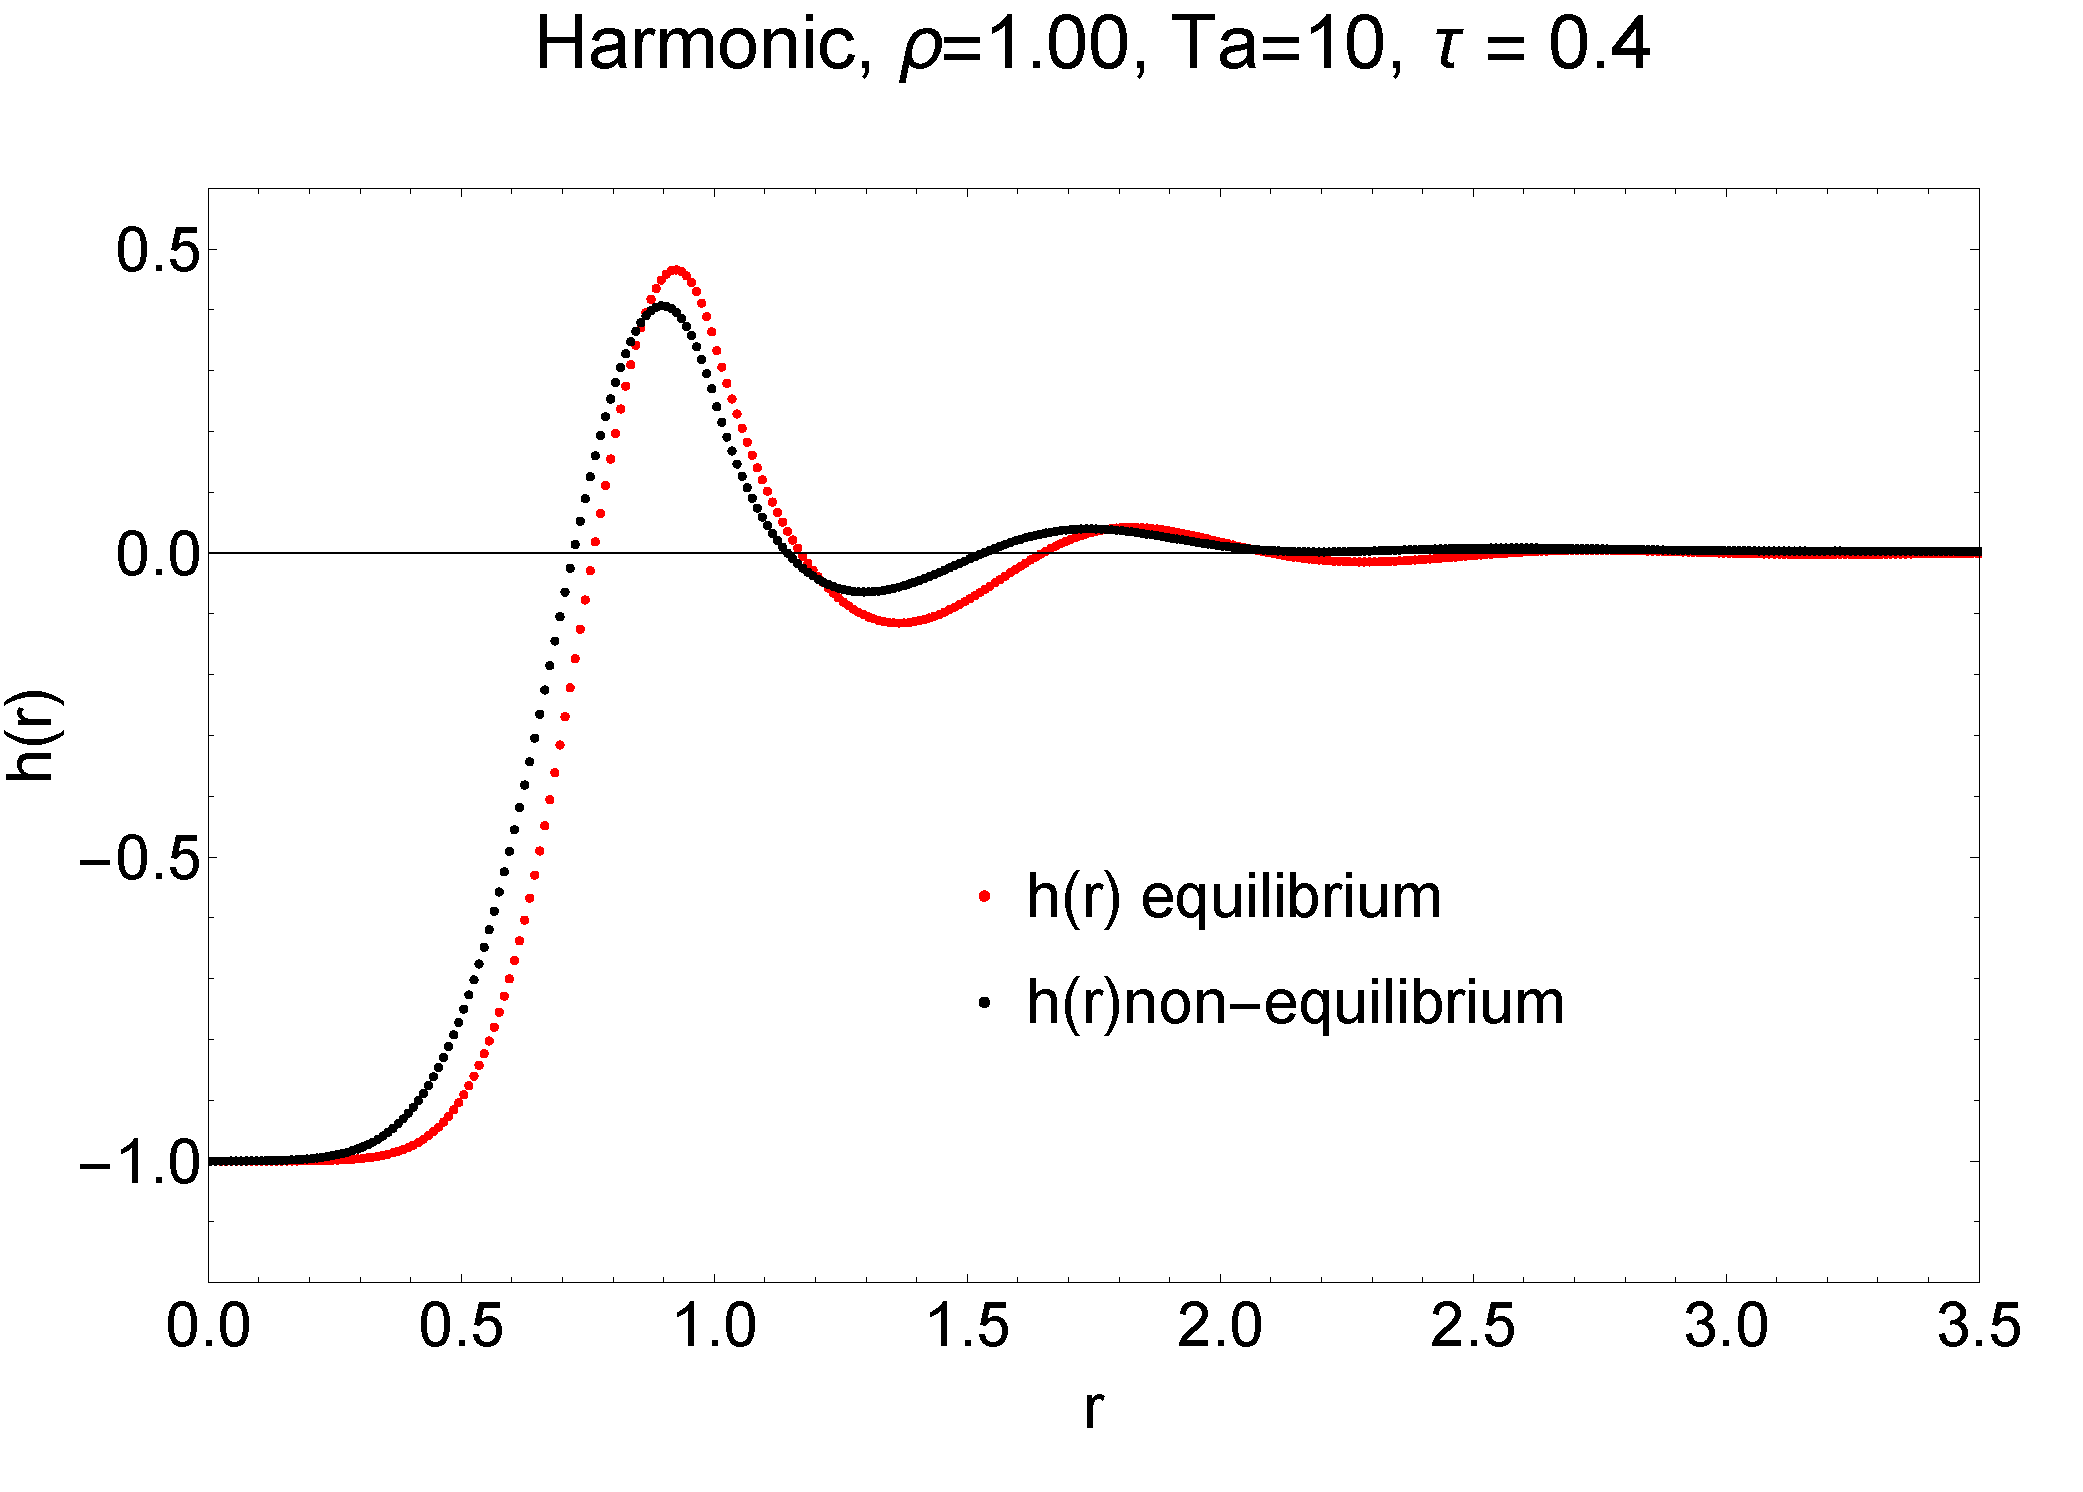
\includegraphics[scale=0.25, clip=True]{HarmonicA16_p1.0_Ta10_U0.40.pdf}
    \caption{}
    \label{Fig:n}
\end{figure}

\begin{figure}
    \centering
    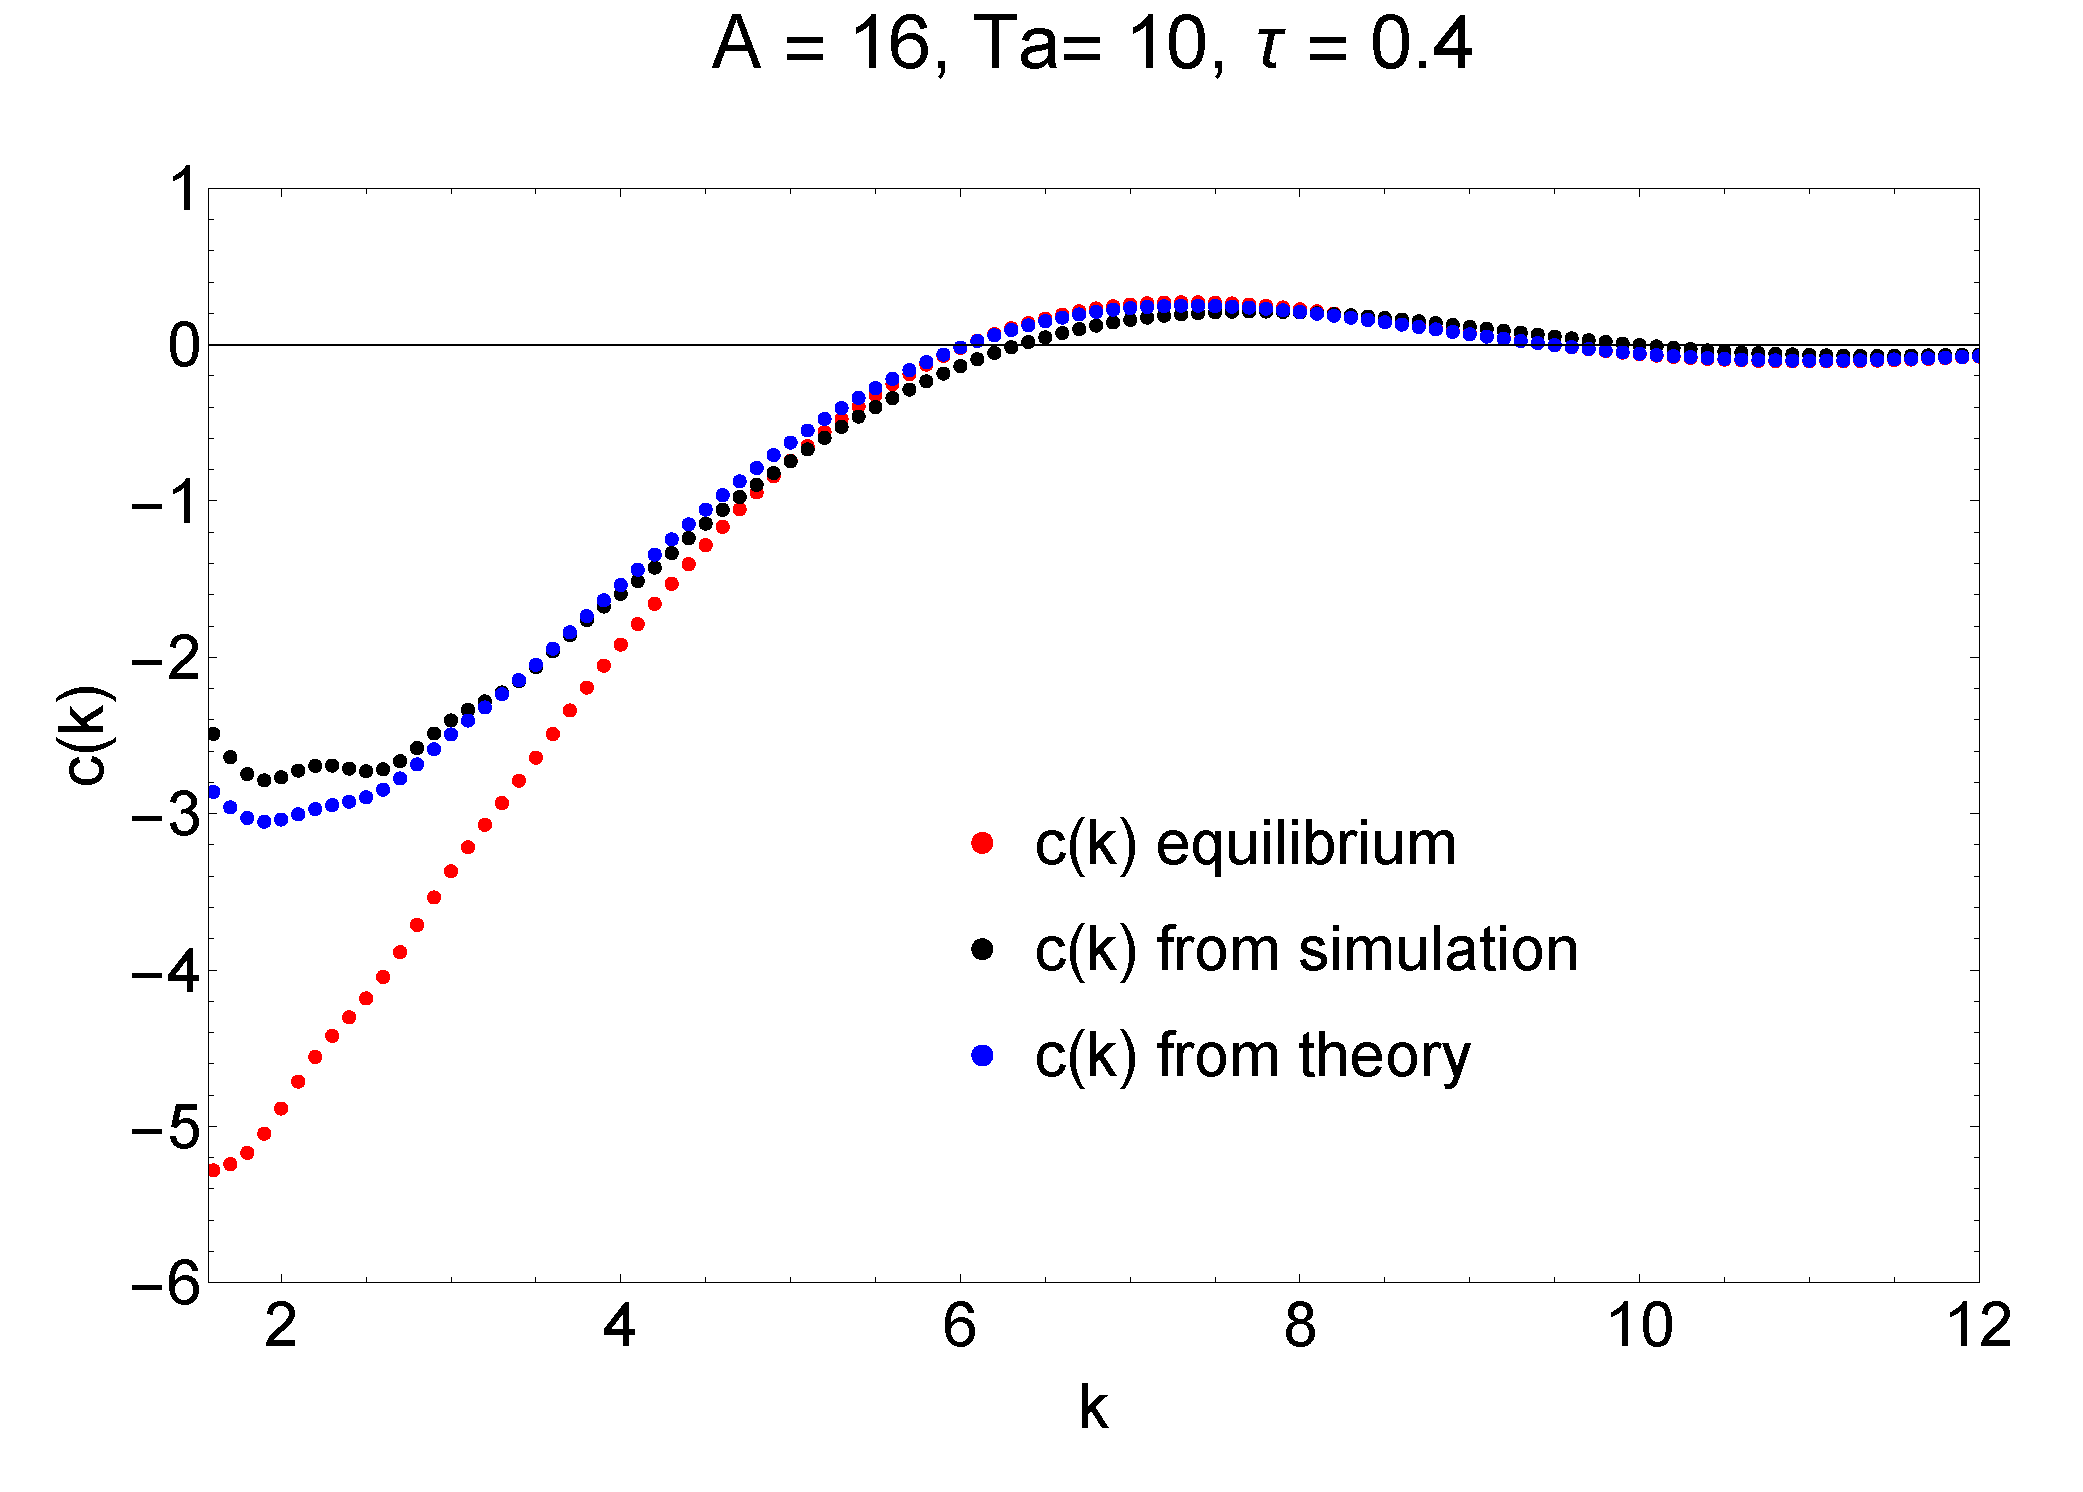
\includegraphics[scale=0.25, clip=True]{Ck_A16_T10_U0.4.pdf}
    \caption{Prediction for c(k) in a moderately driven system of harmonic disk particles following the procedure in the text (blue), compared with predicted c(k) for the system with no driving (red) and measured c(k) from simulation with driving (black). $\rho = 1.00, A = 16, \tau = 0.4, T_A = 10$ (blue, black); $T_A = 0$ (red).}
    \label{Fig:n}
\end{figure}

\begin{figure}
    \centering
    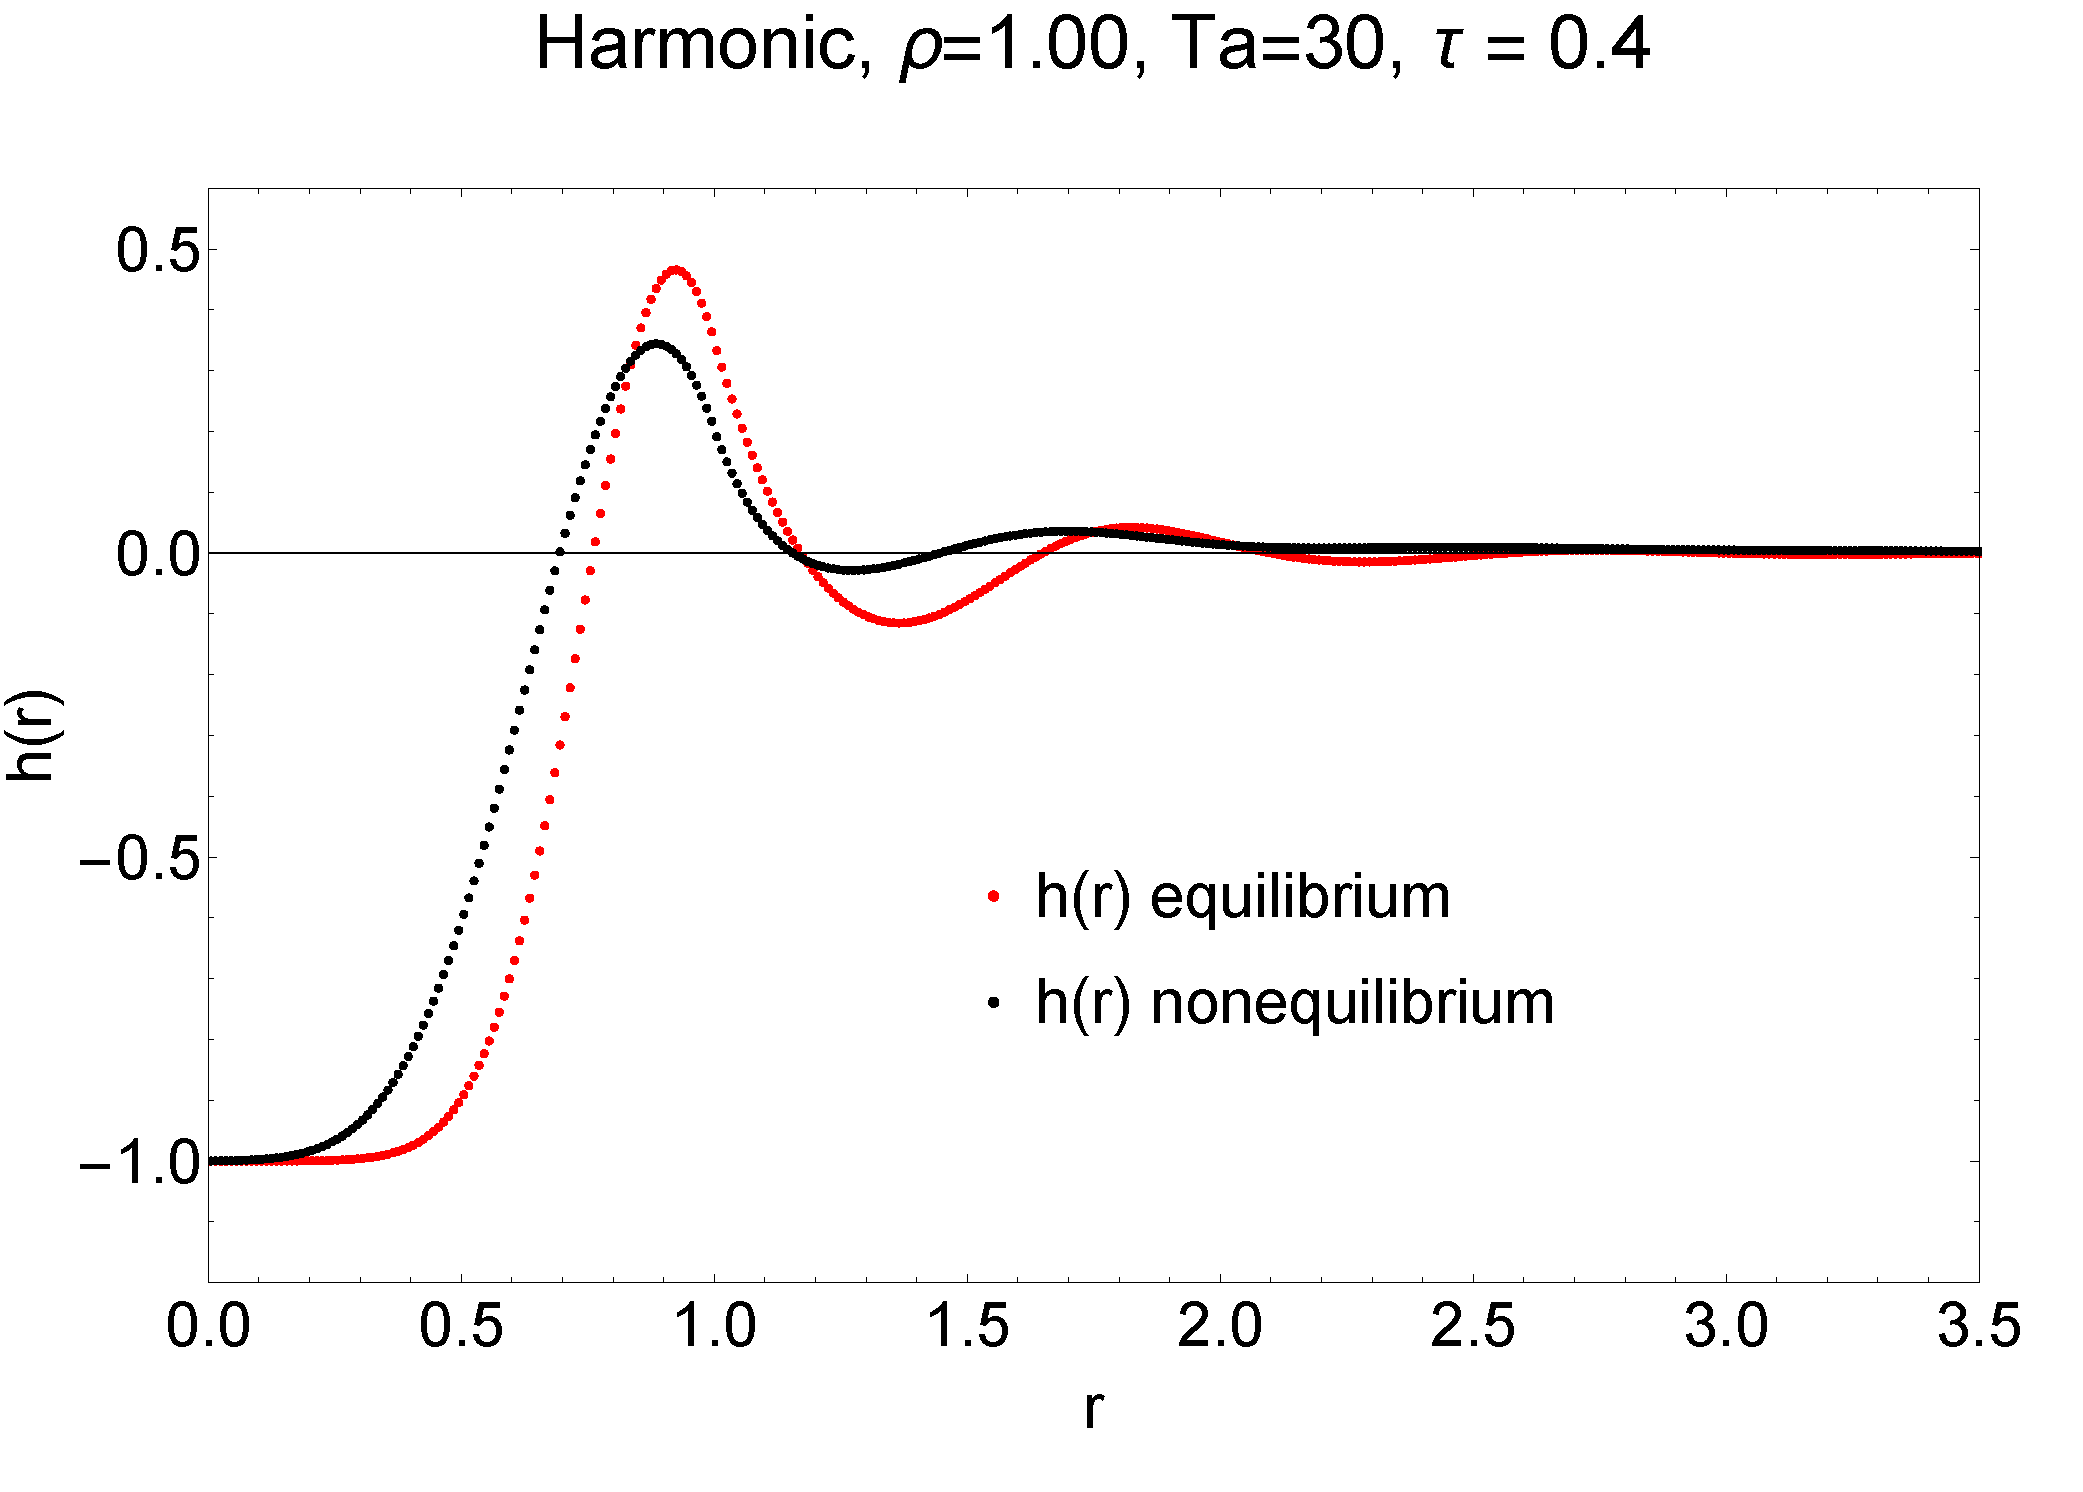
\includegraphics[scale=0.25, clip=True]{HarmonicA16_p1.0_Ta30_U0.40.pdf}
    \caption{}
    \label{Fig:n}
\end{figure}

\begin{figure}
    \centering
    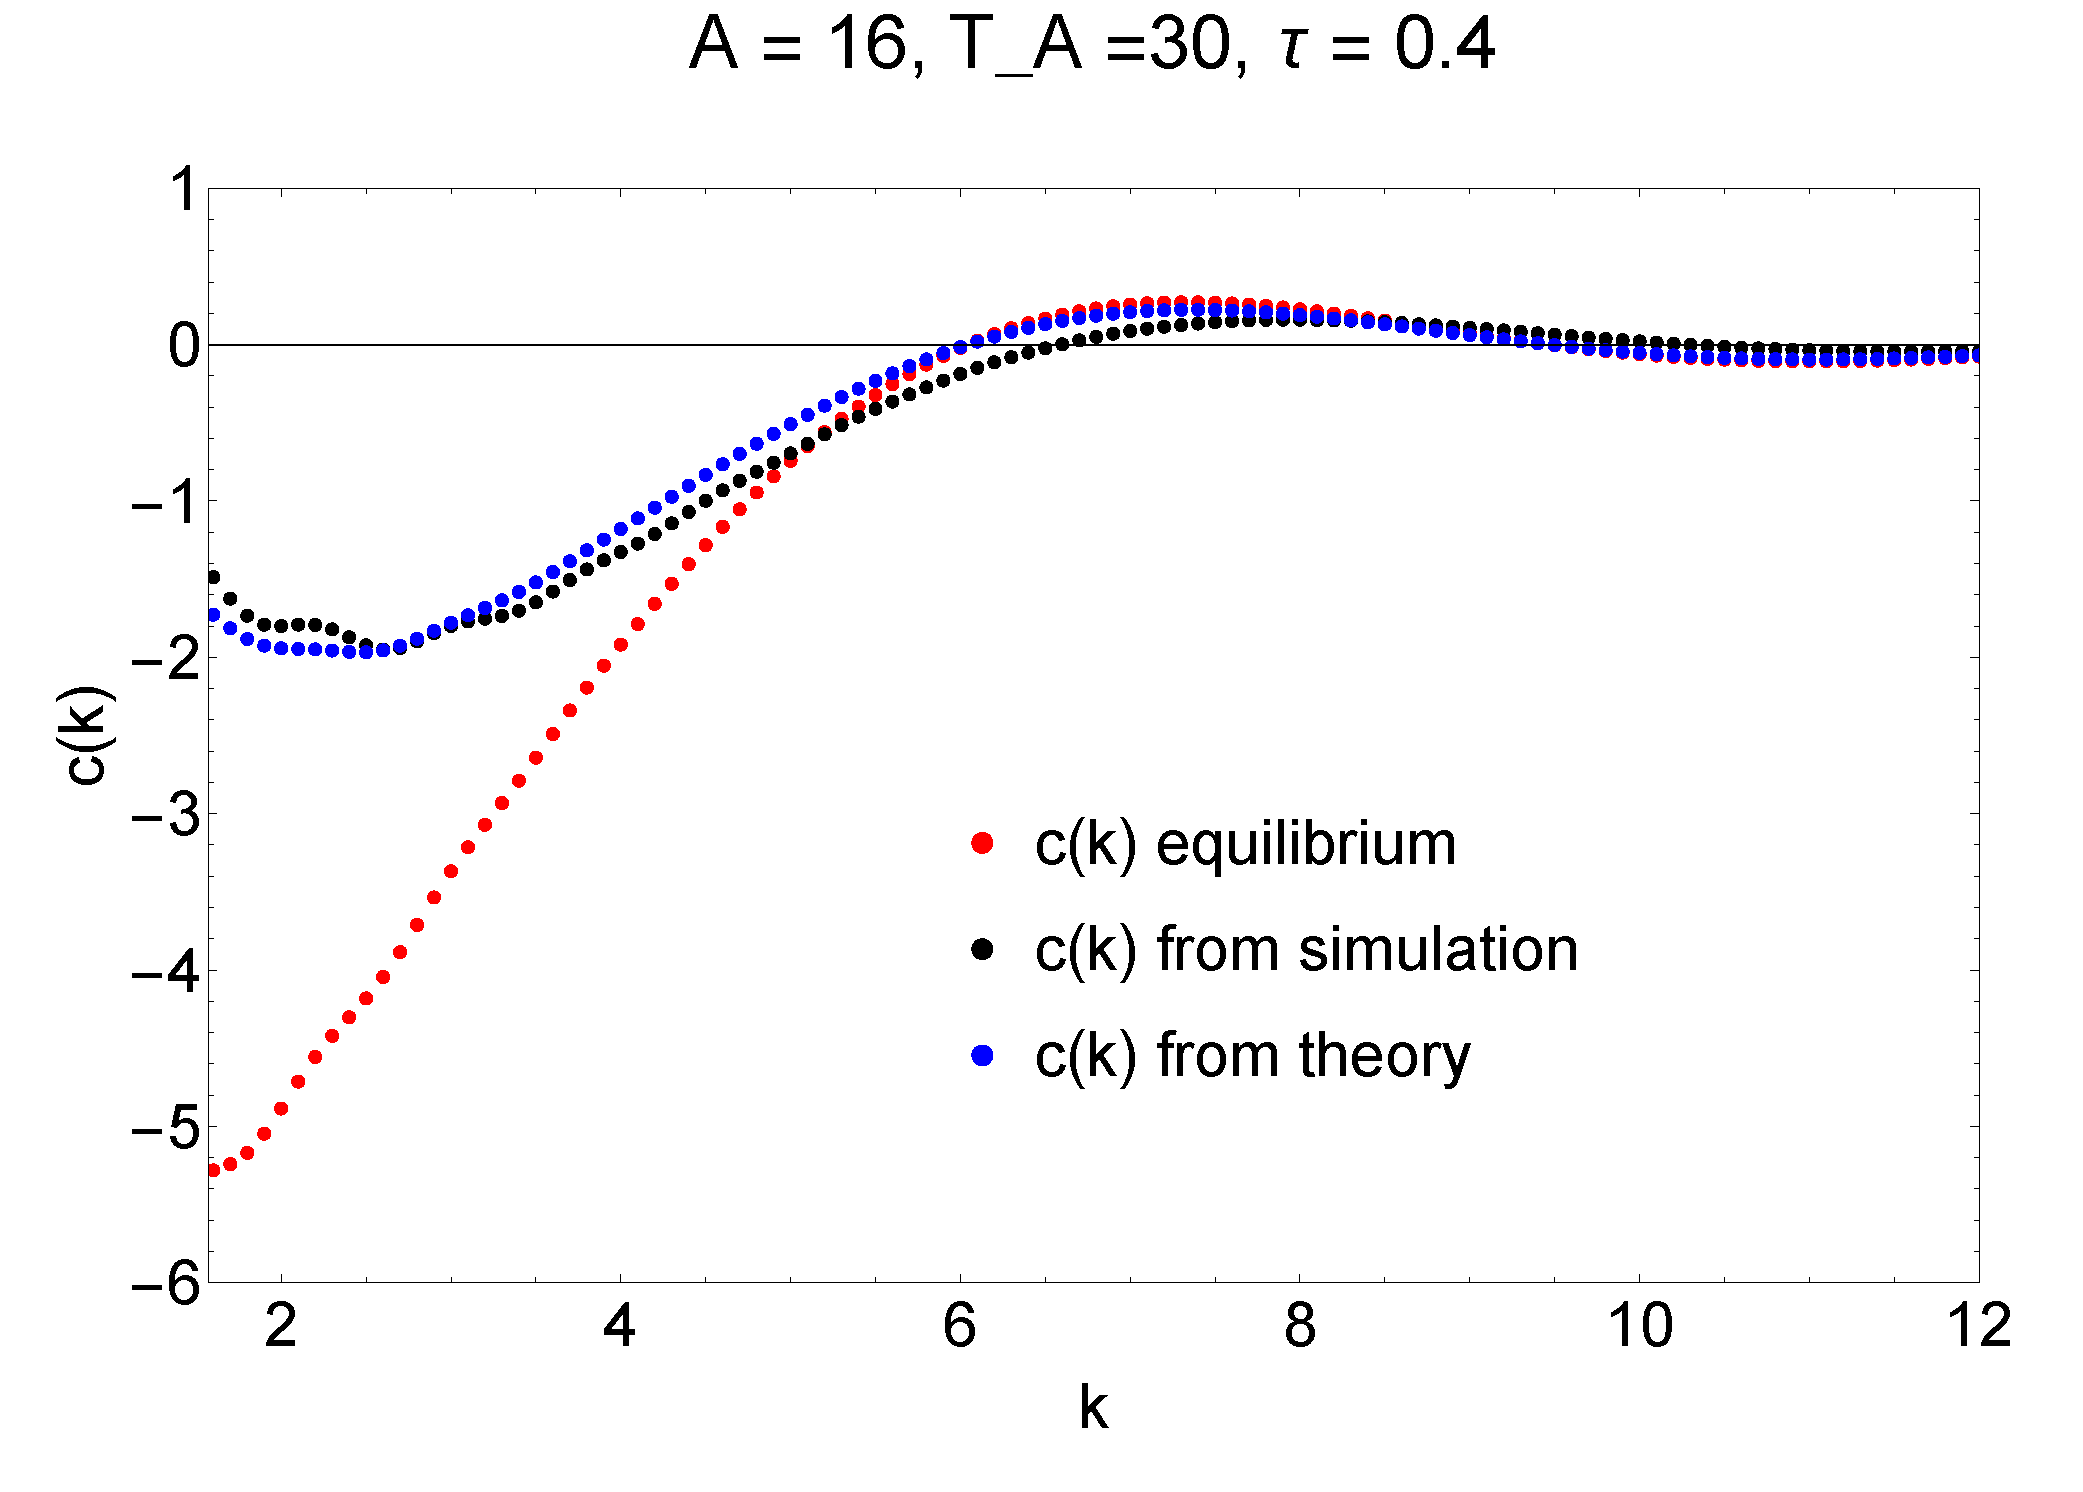
\includegraphics[scale=0.25, clip=True]{Ck_A16_T30_U0.4.pdf}
    \caption{Prediction for c(k) in a strongly driven system of harmonic disk particles (blue), compared with predicted c(k) for the system with no driving (red) and measured c(k) from simulation with driving (black). $\rho = 1.00, A = 16, \tau = 0.4, T_A = 30$ (blue, black); $T_A = 0$ (red).}
    \label{Fig:n}
\end{figure}

\begin{figure}
    \centering
    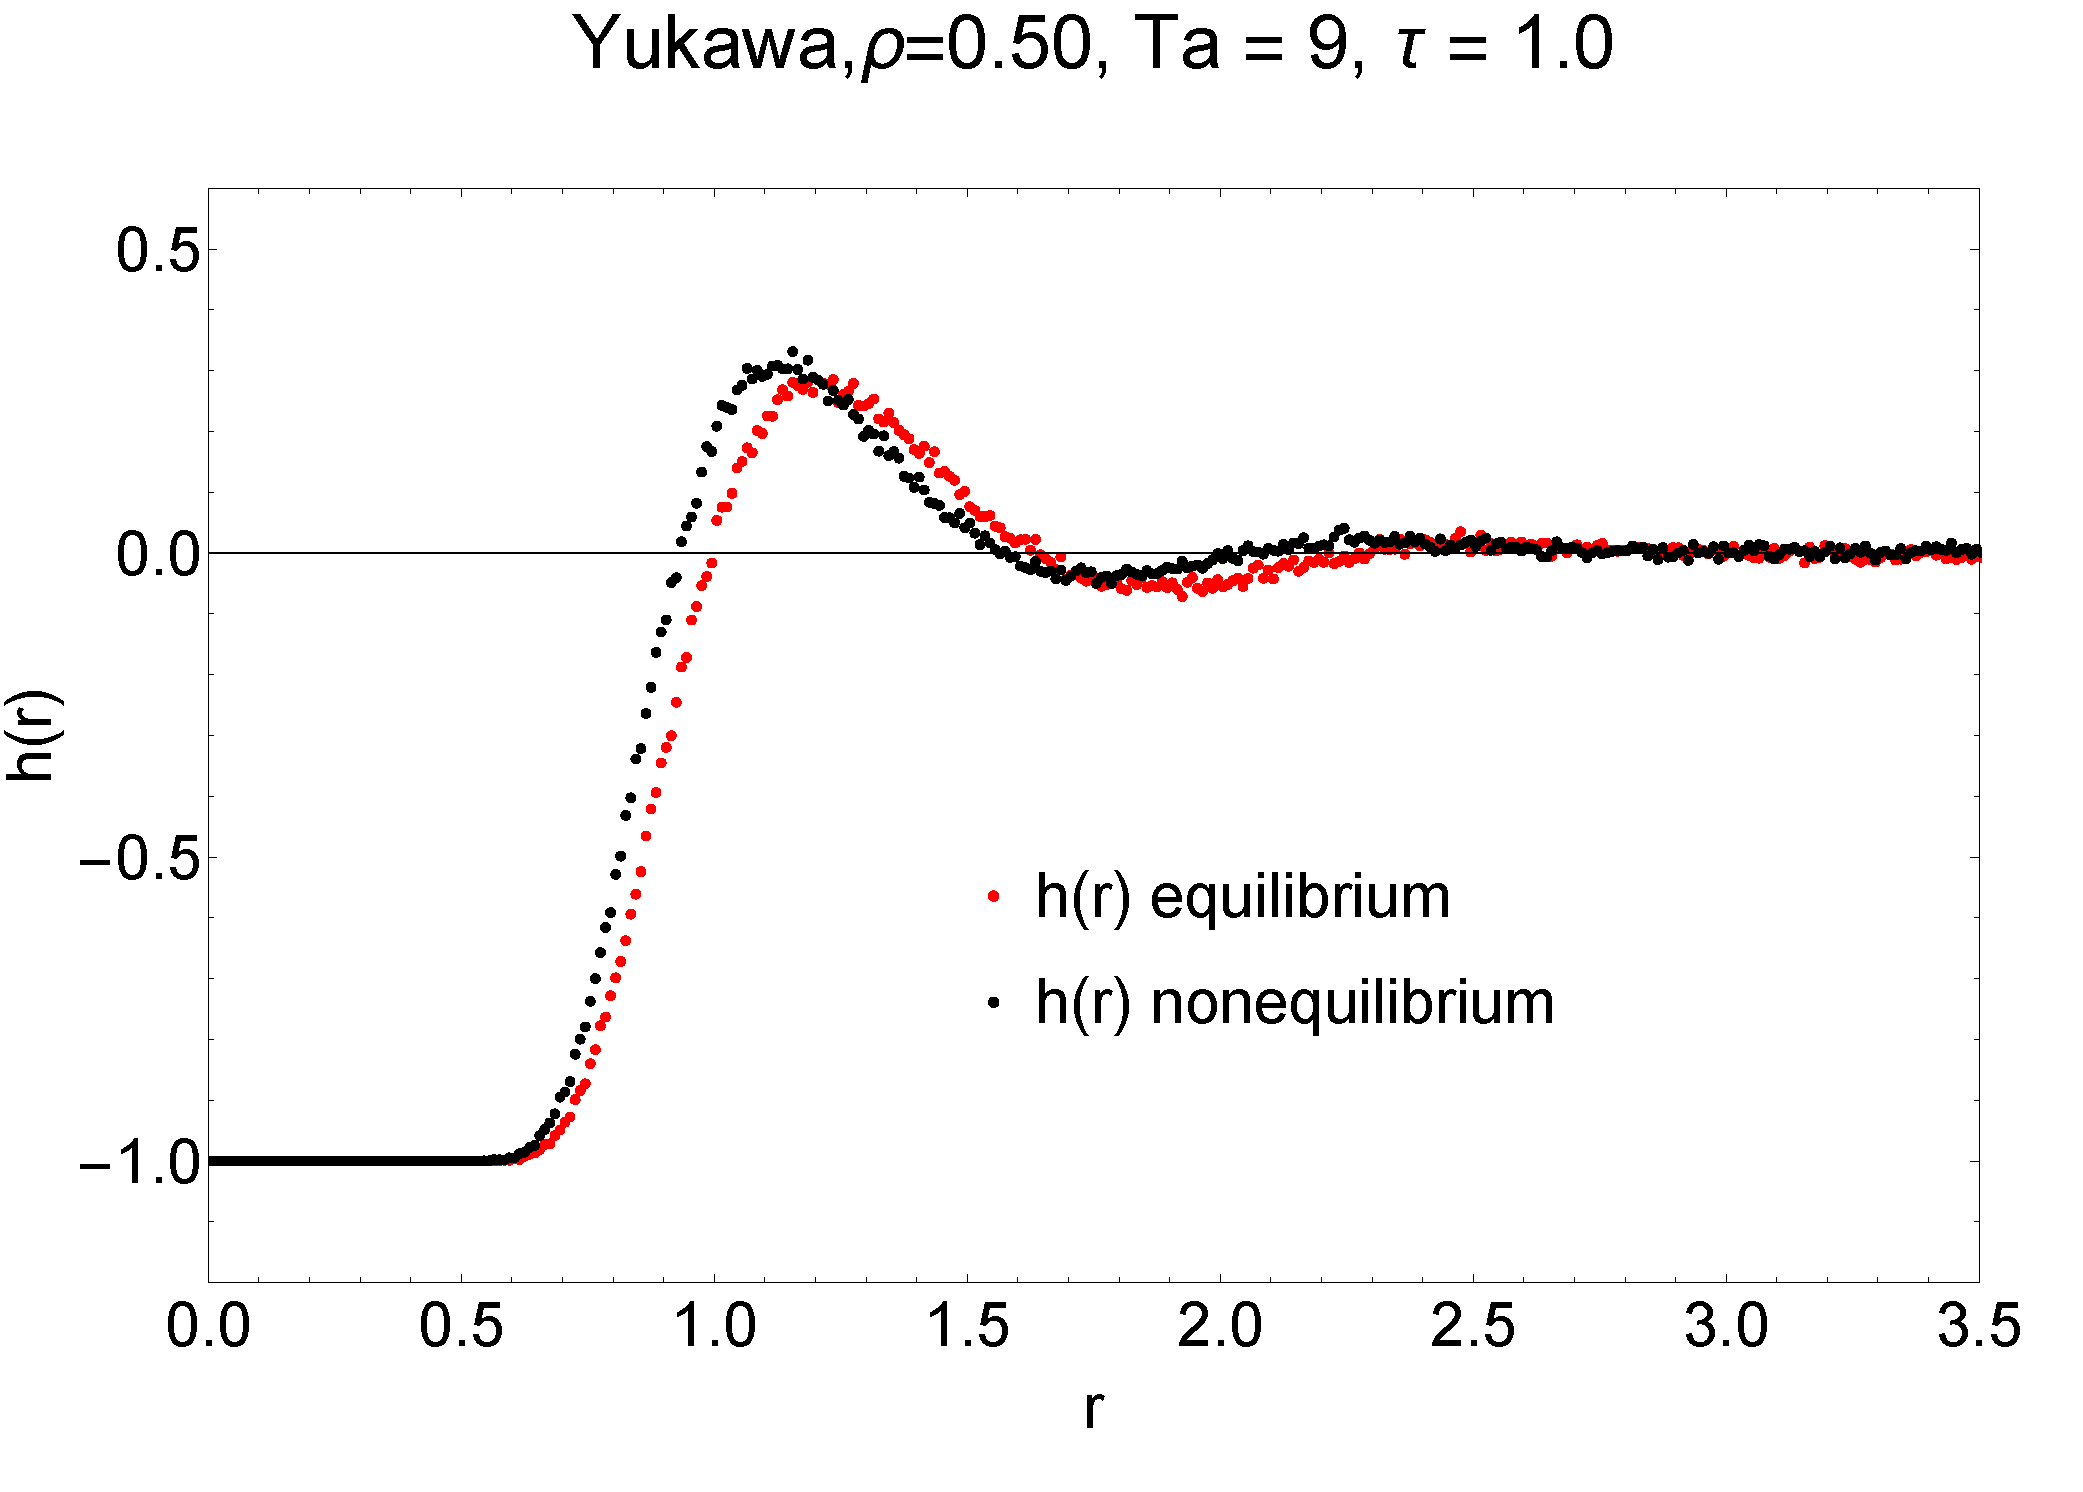
\includegraphics[scale=0.25, clip=True]{Yukawahr_Yp0.5_Pe3_U1.00.pdf}
    \caption{}
    \label{Fig:n}
\end{figure}

\begin{figure}
    \centering
    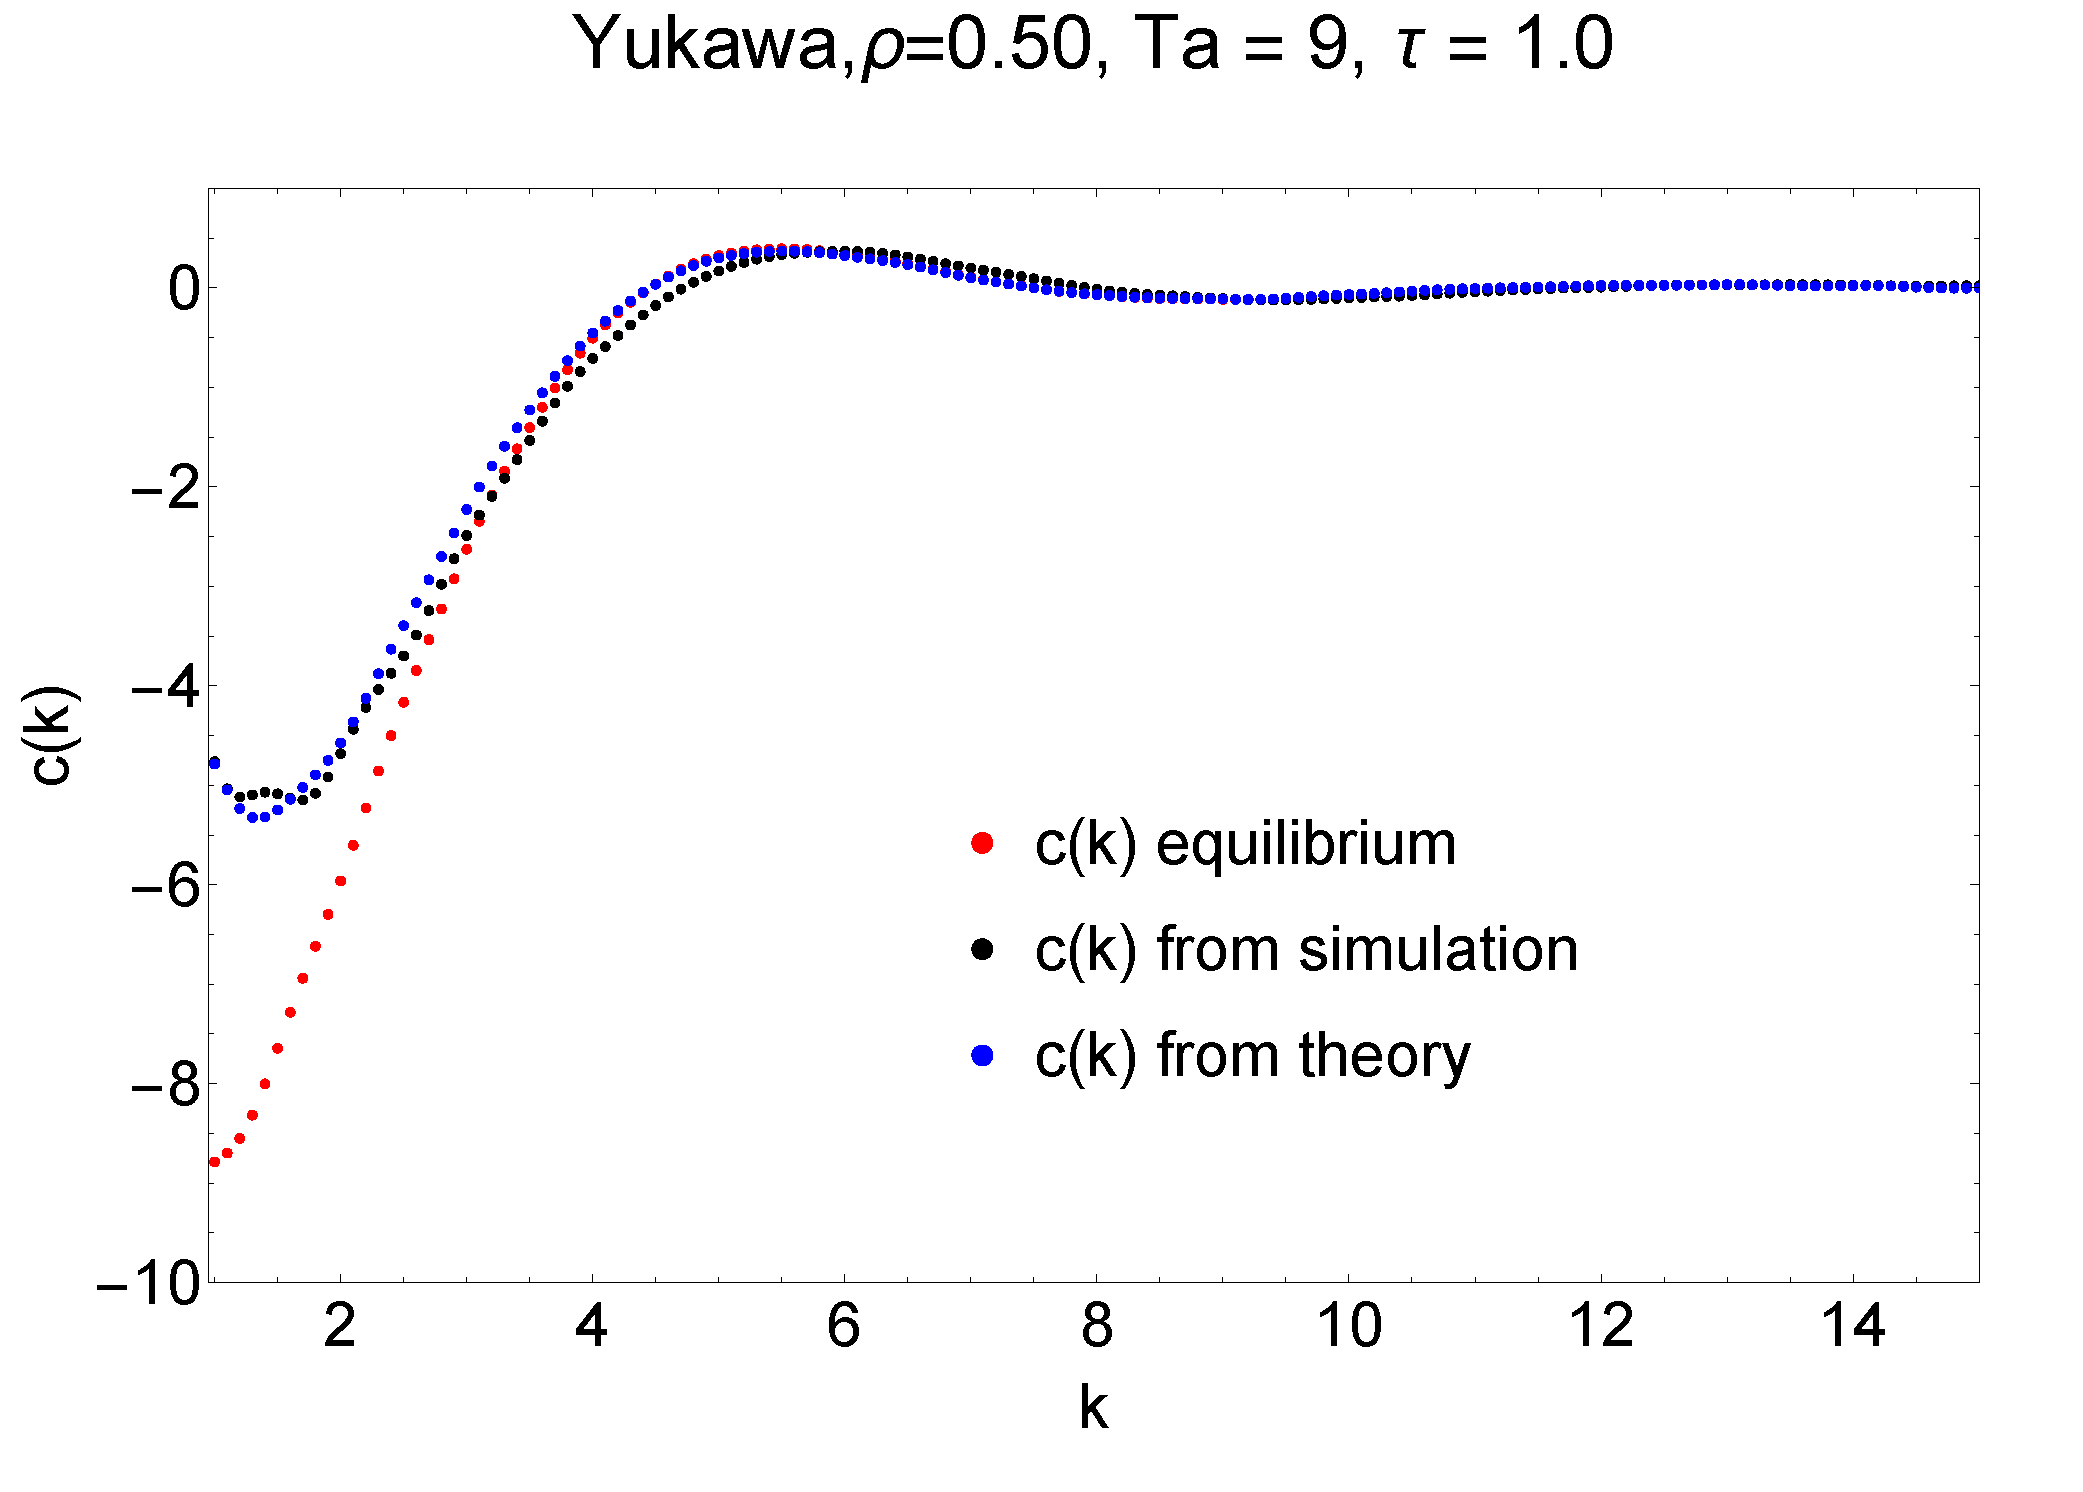
\includegraphics[scale=0.25, clip=True]{YukawaCk_Yp0.5_Pe3_U1.00.pdf}
    \caption{Prediction for c(k) in a moderately driven system of Yukawa particles (blue), compared with predicted c(k) for the system with no driving (red) and measured c(k) from simulation with driving (black). $\rho = 0.50, A = 50, \kappa = 4.00, \tau = 1.0, T_A = 9$ (blue, black); $T_A = 0$ (red).}
    \label{Fig:n}
\end{figure}

\begin{figure}
    \centering
    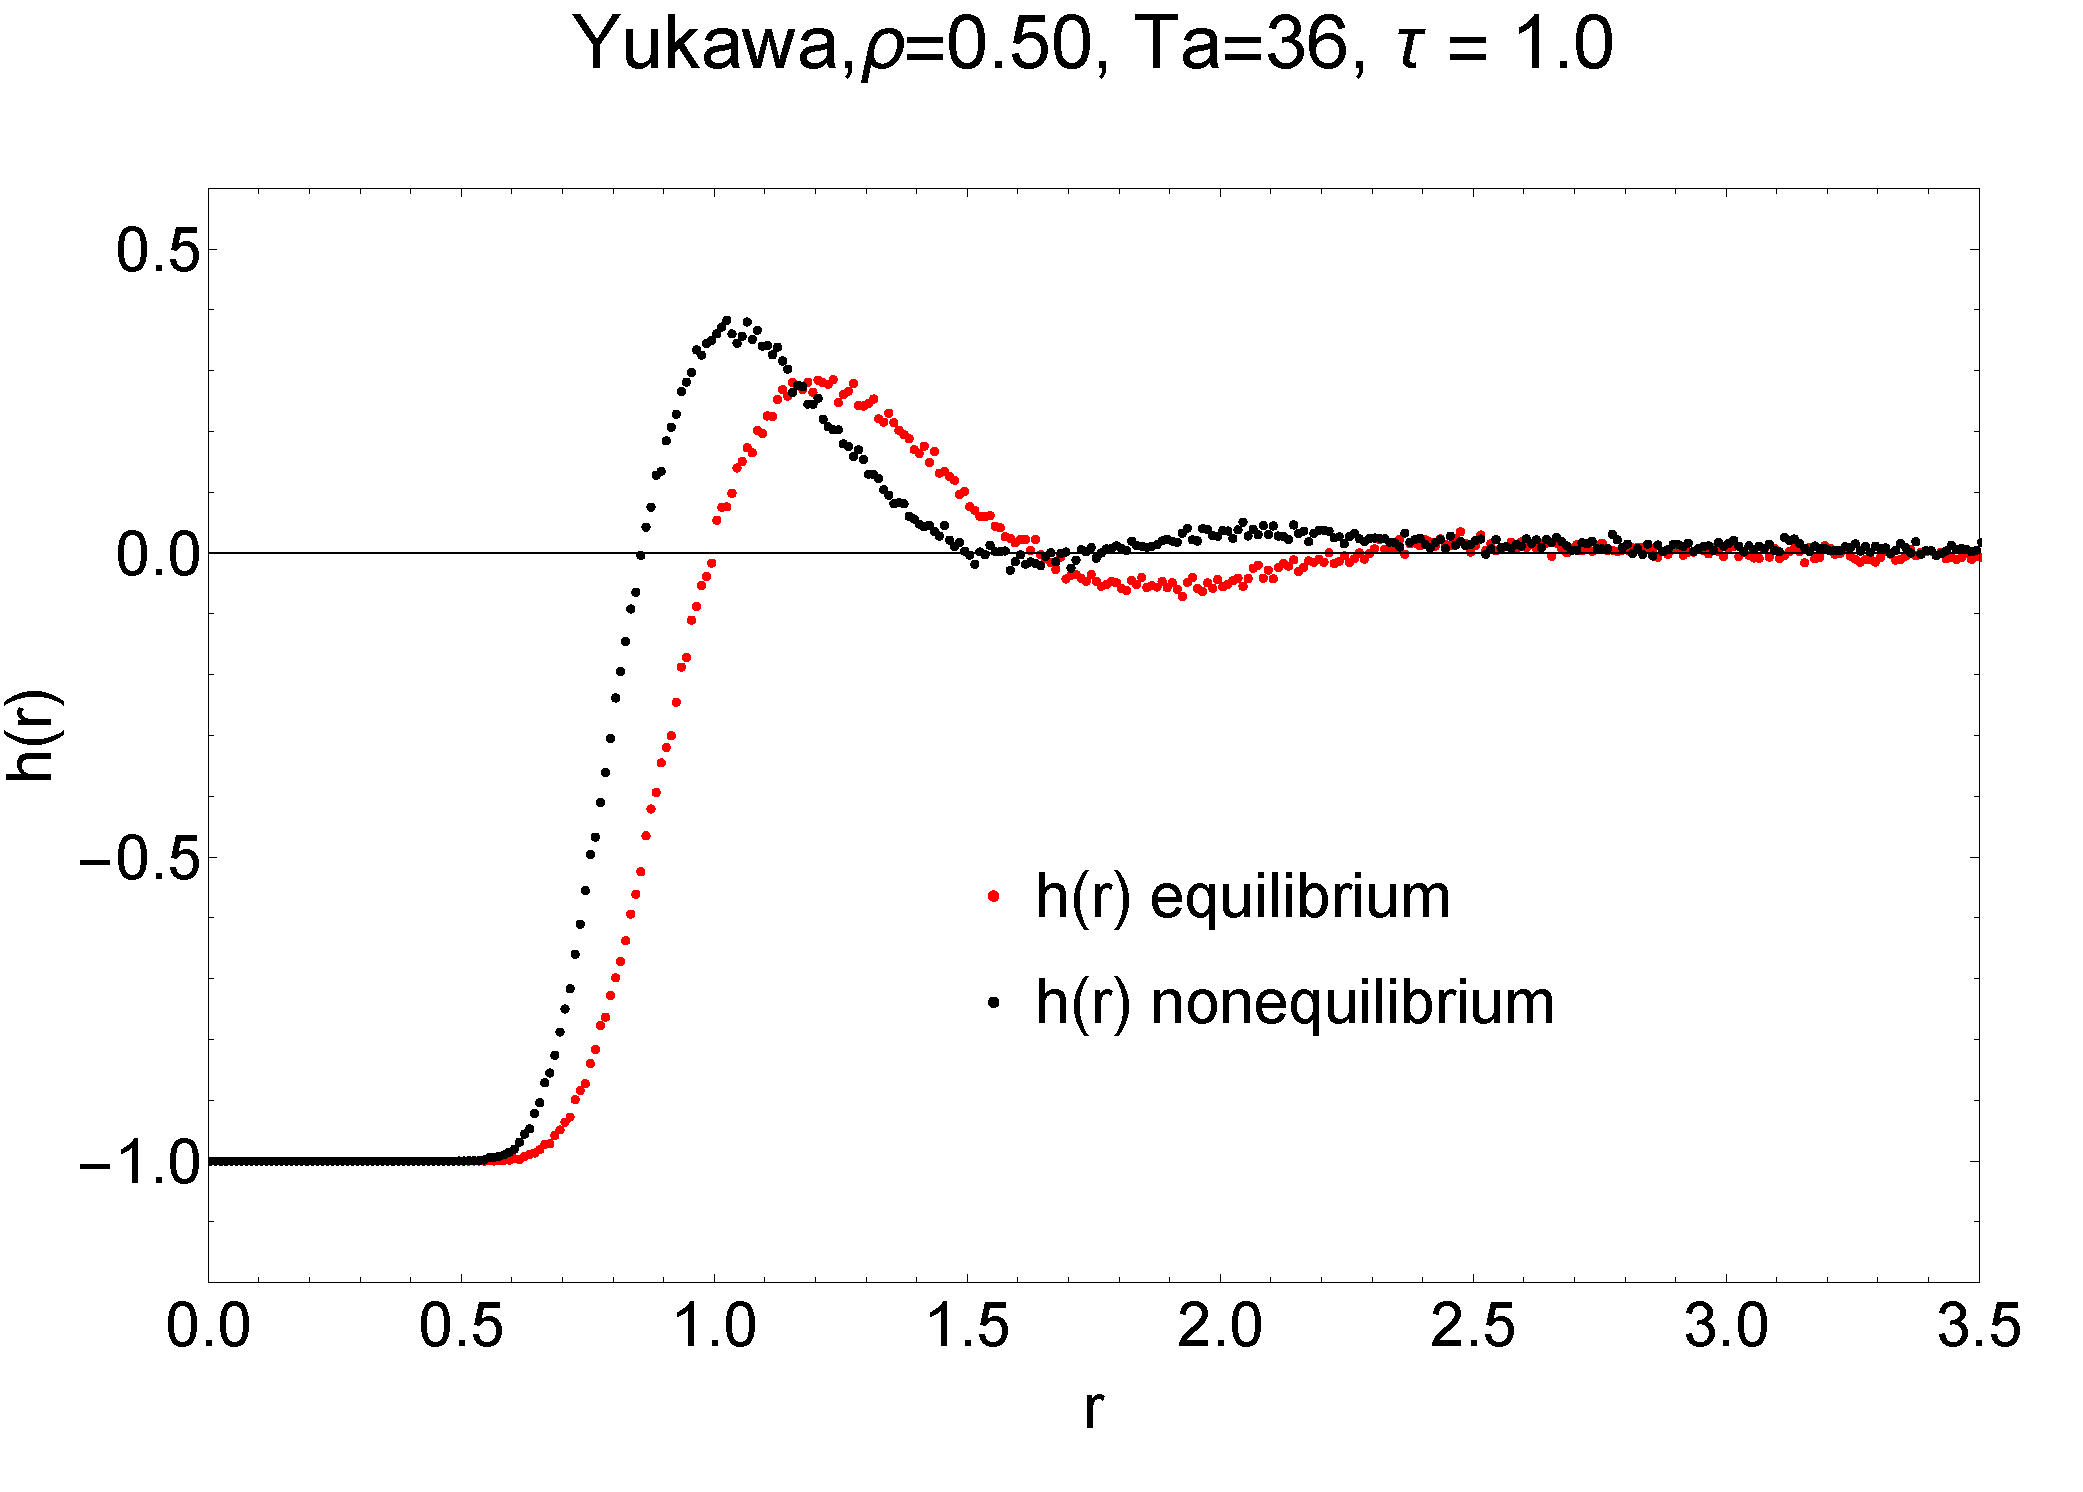
\includegraphics[scale=0.25, clip=True]{Yukawahr_Yp0.5_Pe6_U1.00.pdf}
    \caption{}
    \label{Fig:n}
\end{figure}

\begin{figure}
    \centering
    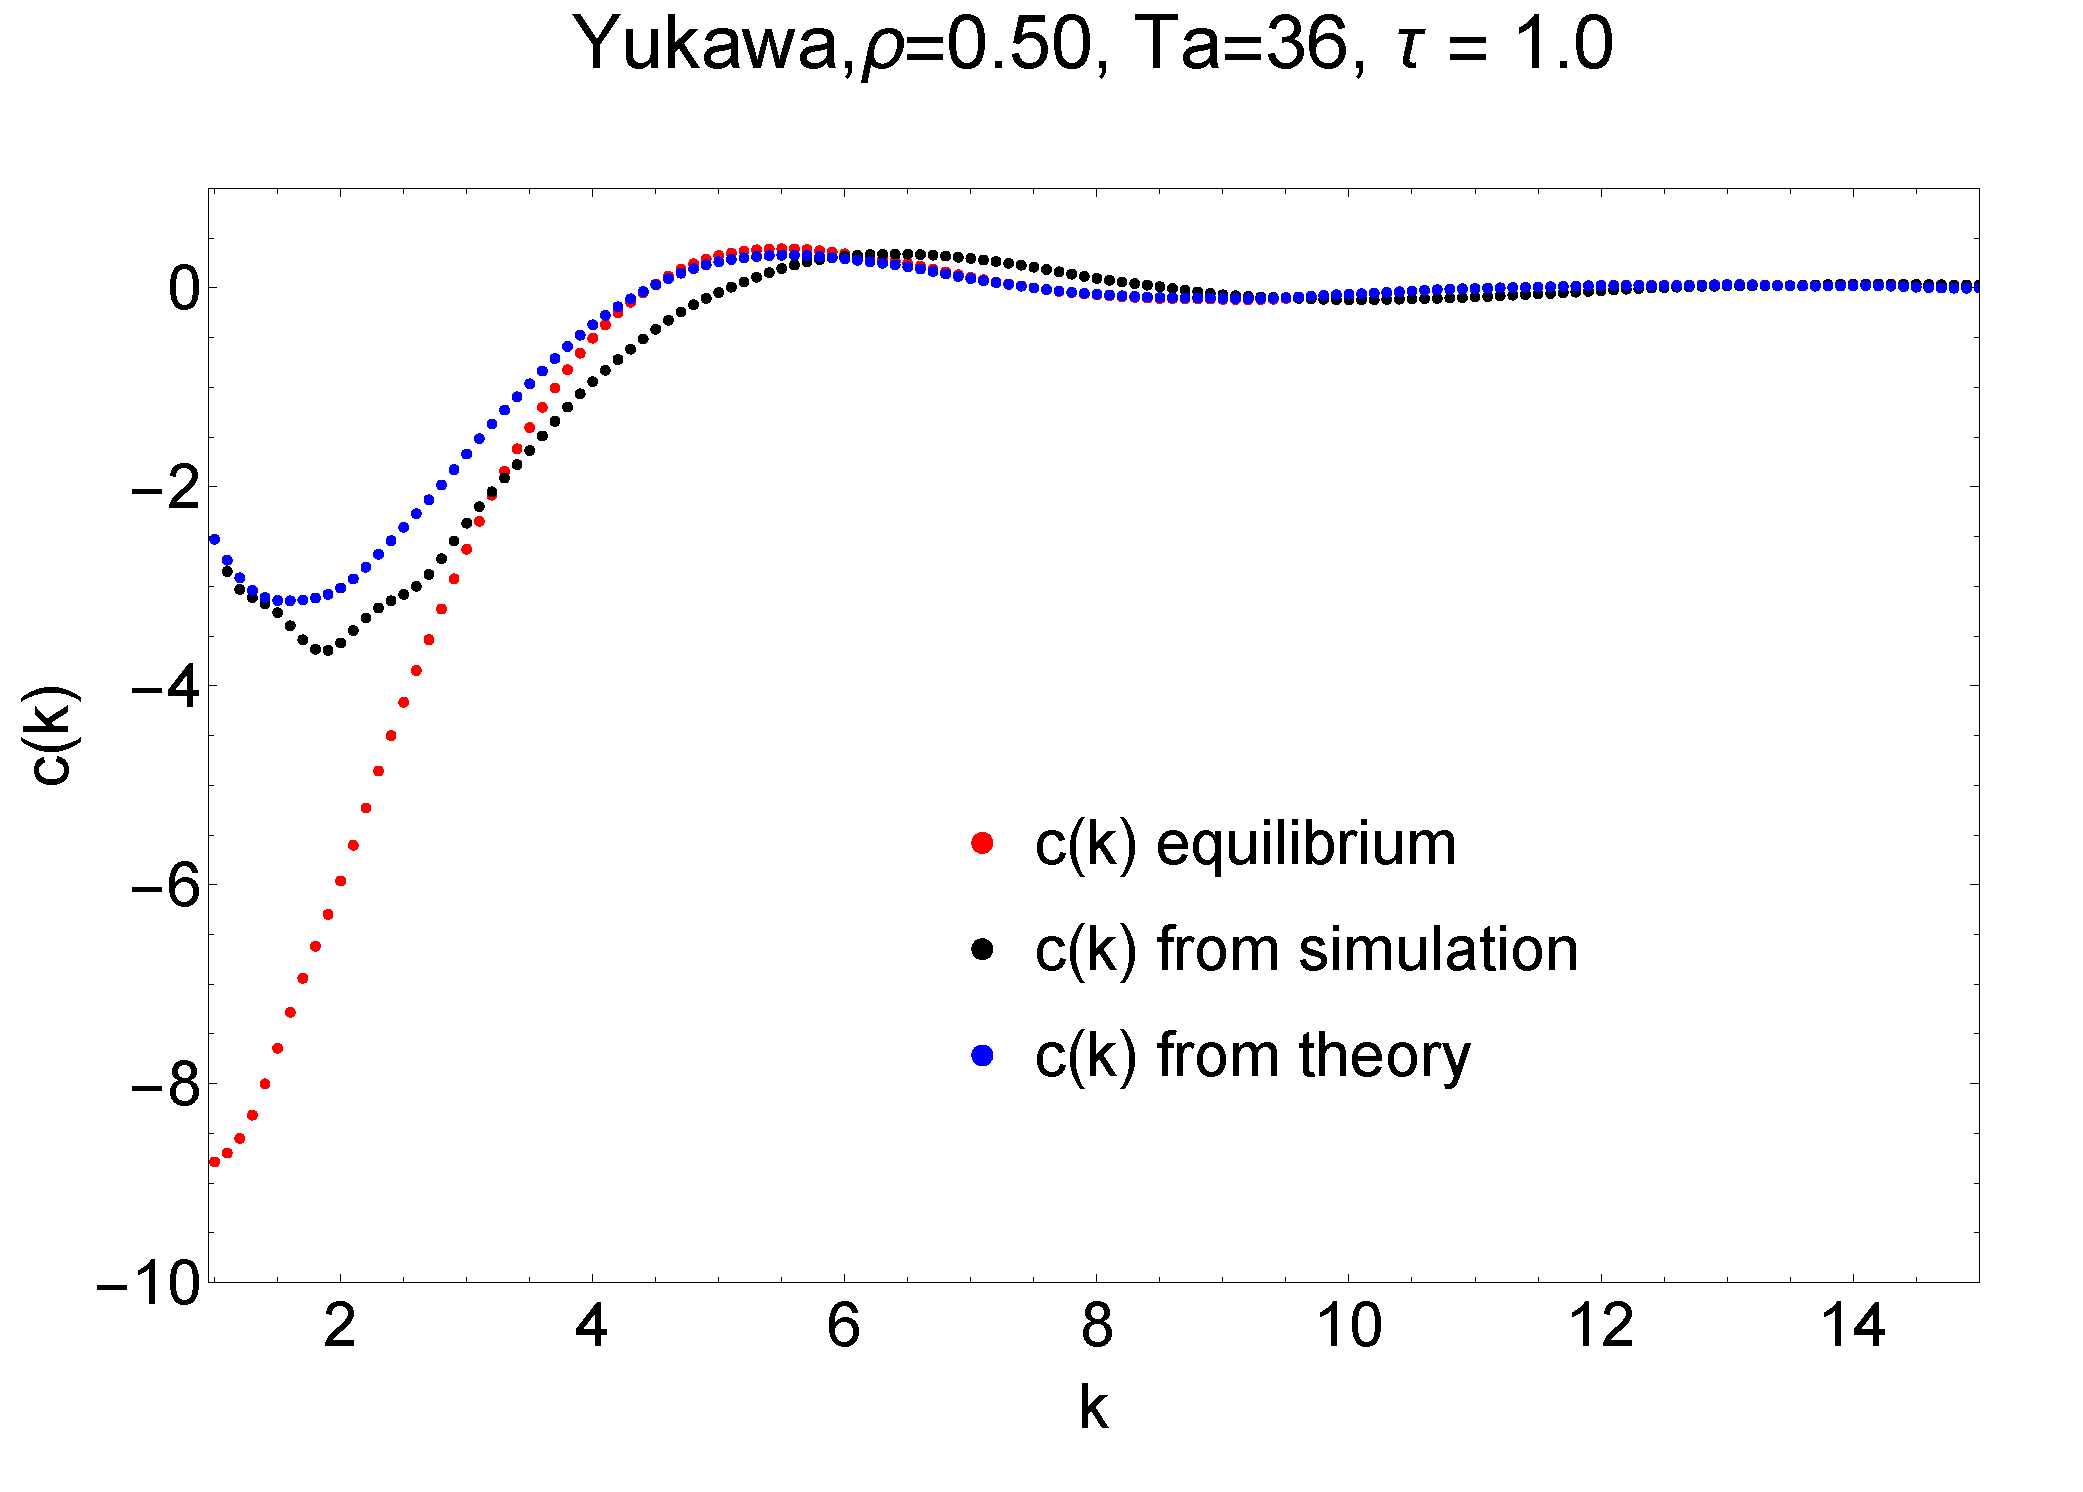
\includegraphics[scale=0.25, clip=True]{YukawaCk_Yp0.5_Pe6_U1.00.pdf}
    \caption{Prediction for c(k) in a strongly driven system of Yukawa particles (blue), compared with predicted c(k) for the system with no driving (red) and measured c(k) from simulation with driving (black). $\rho = 0.50, A = 50, \kappa = 4.00, \tau = 1.0, T_A = 36$ (blue, black); $T_A = 0$ (red).}
    \label{Fig:n}
\end{figure}

\begin{figure}
    \centering
    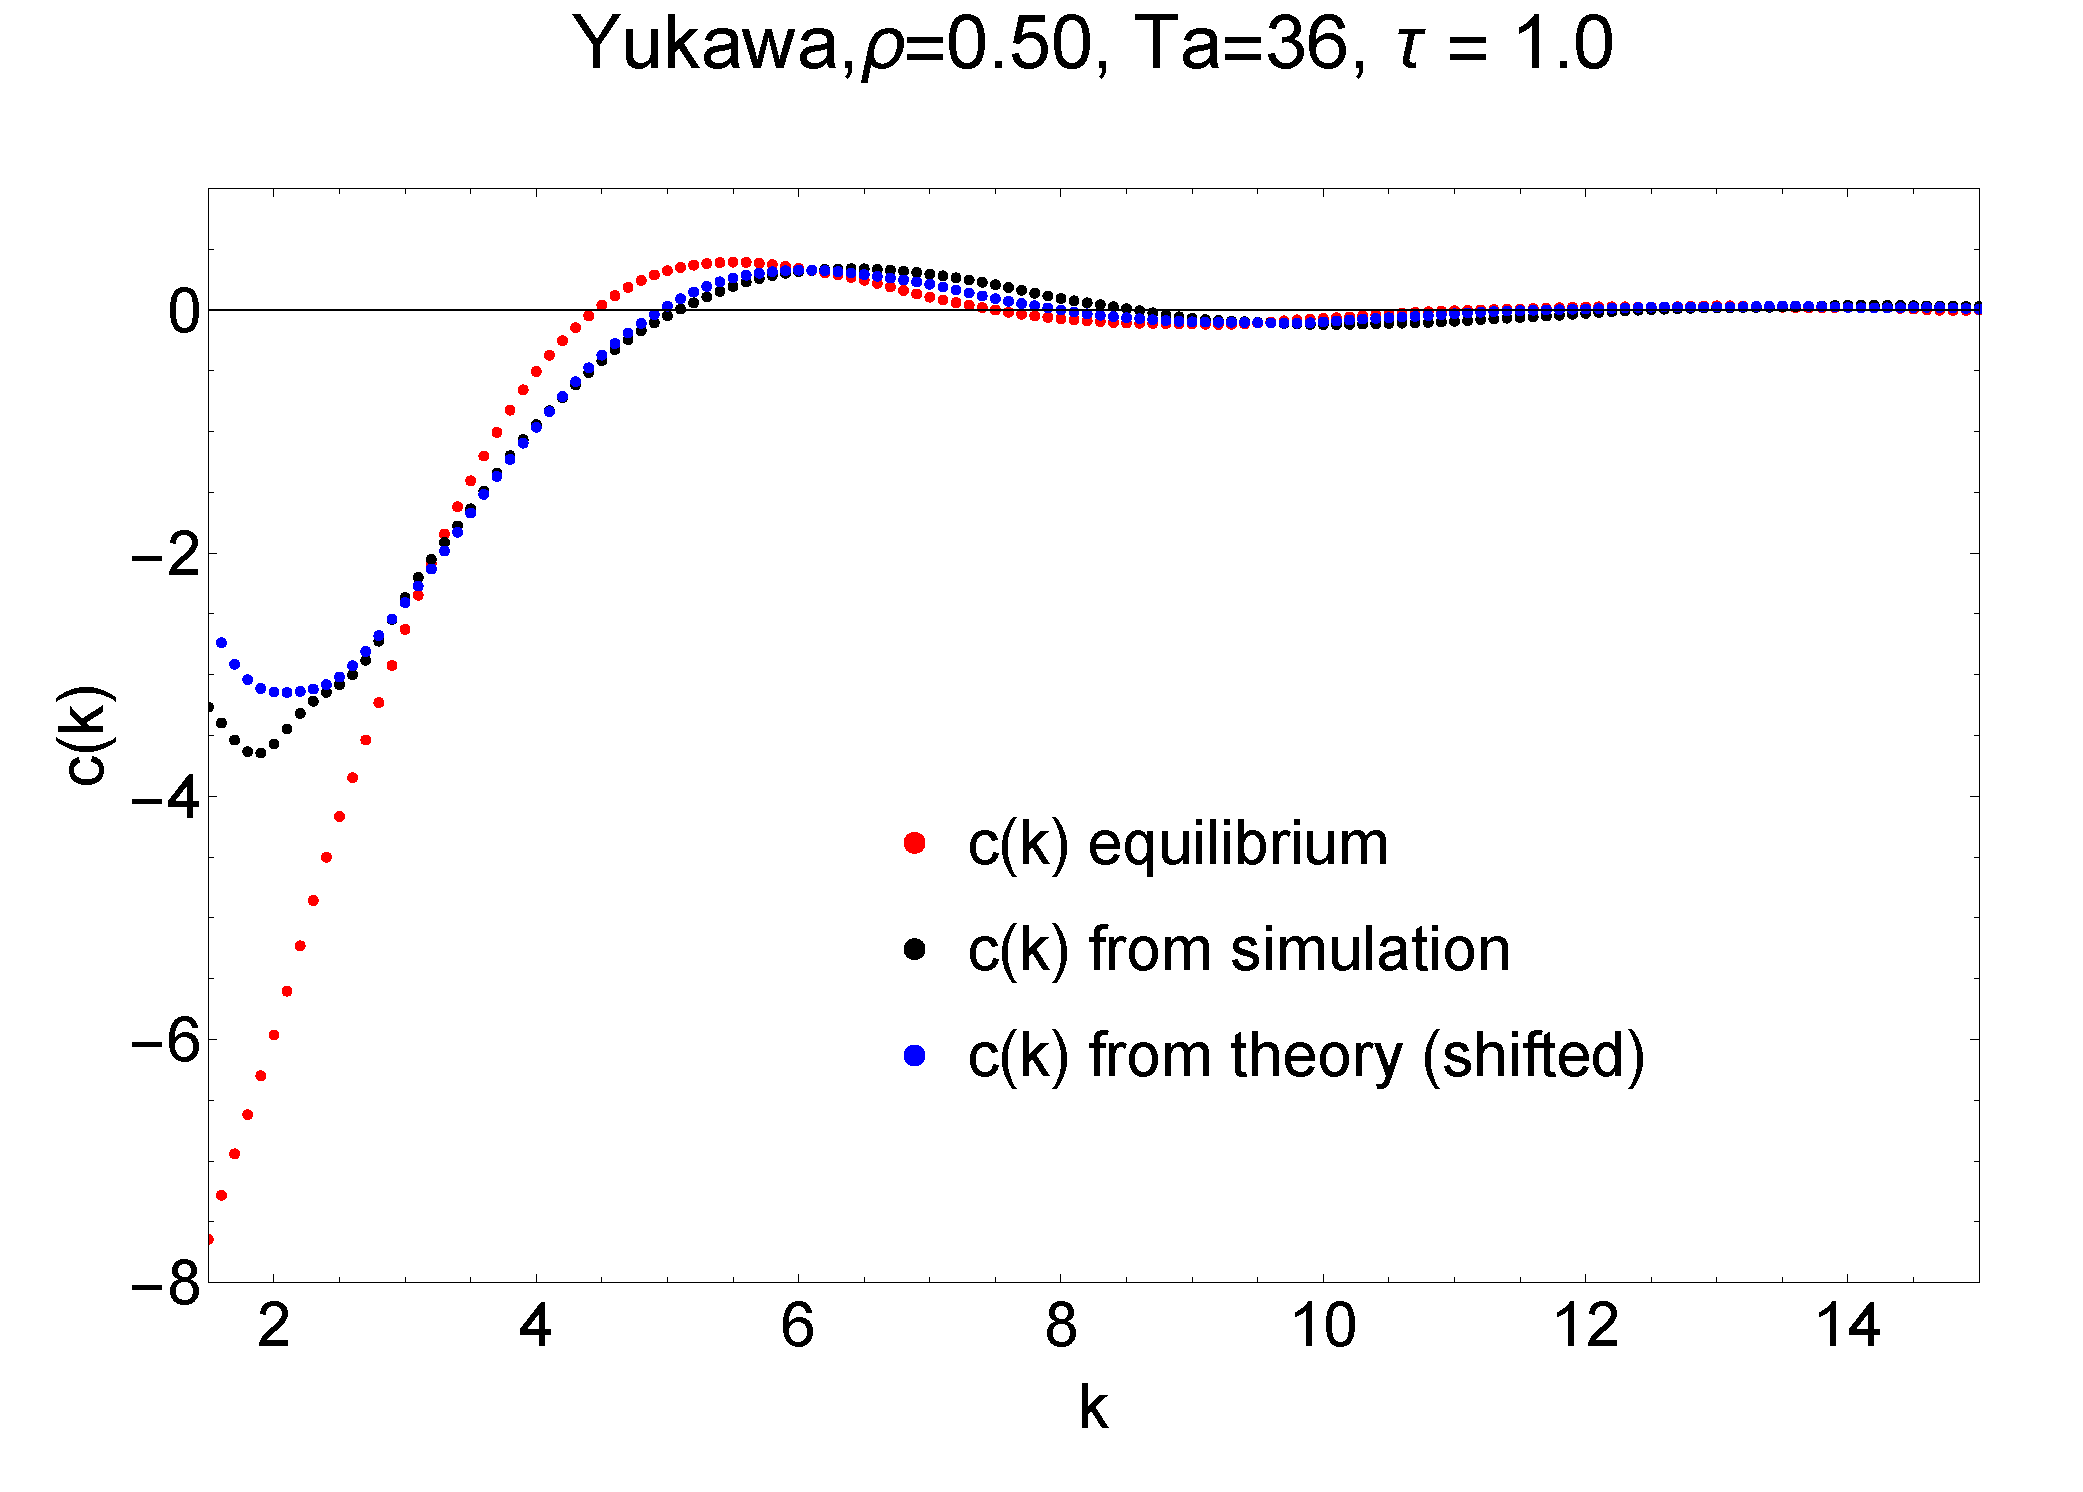
\includegraphics[scale=0.25, clip=True]{ShiftedYukawaCk_Yp0.5_Pe6_U1.00.pdf}
    \caption{Prediction for c(k) in a strongly driven system of Yukawa particles (blue), compared with predicted c(k) for the system with no driving (red) and measured c(k) from simulation with driving (black). Compared with Fig. 8, the theoretical c(k) has along the k axis to alignat with simulation results. $\rho = 0.50, A = 50, \kappa = 4.00, \tau = 1.0, T_A = 36$ (blue, black); $T_A = 0$ (red).}
    \label{Fig:n}
\end{figure}

\begin{figure}
    \centering
    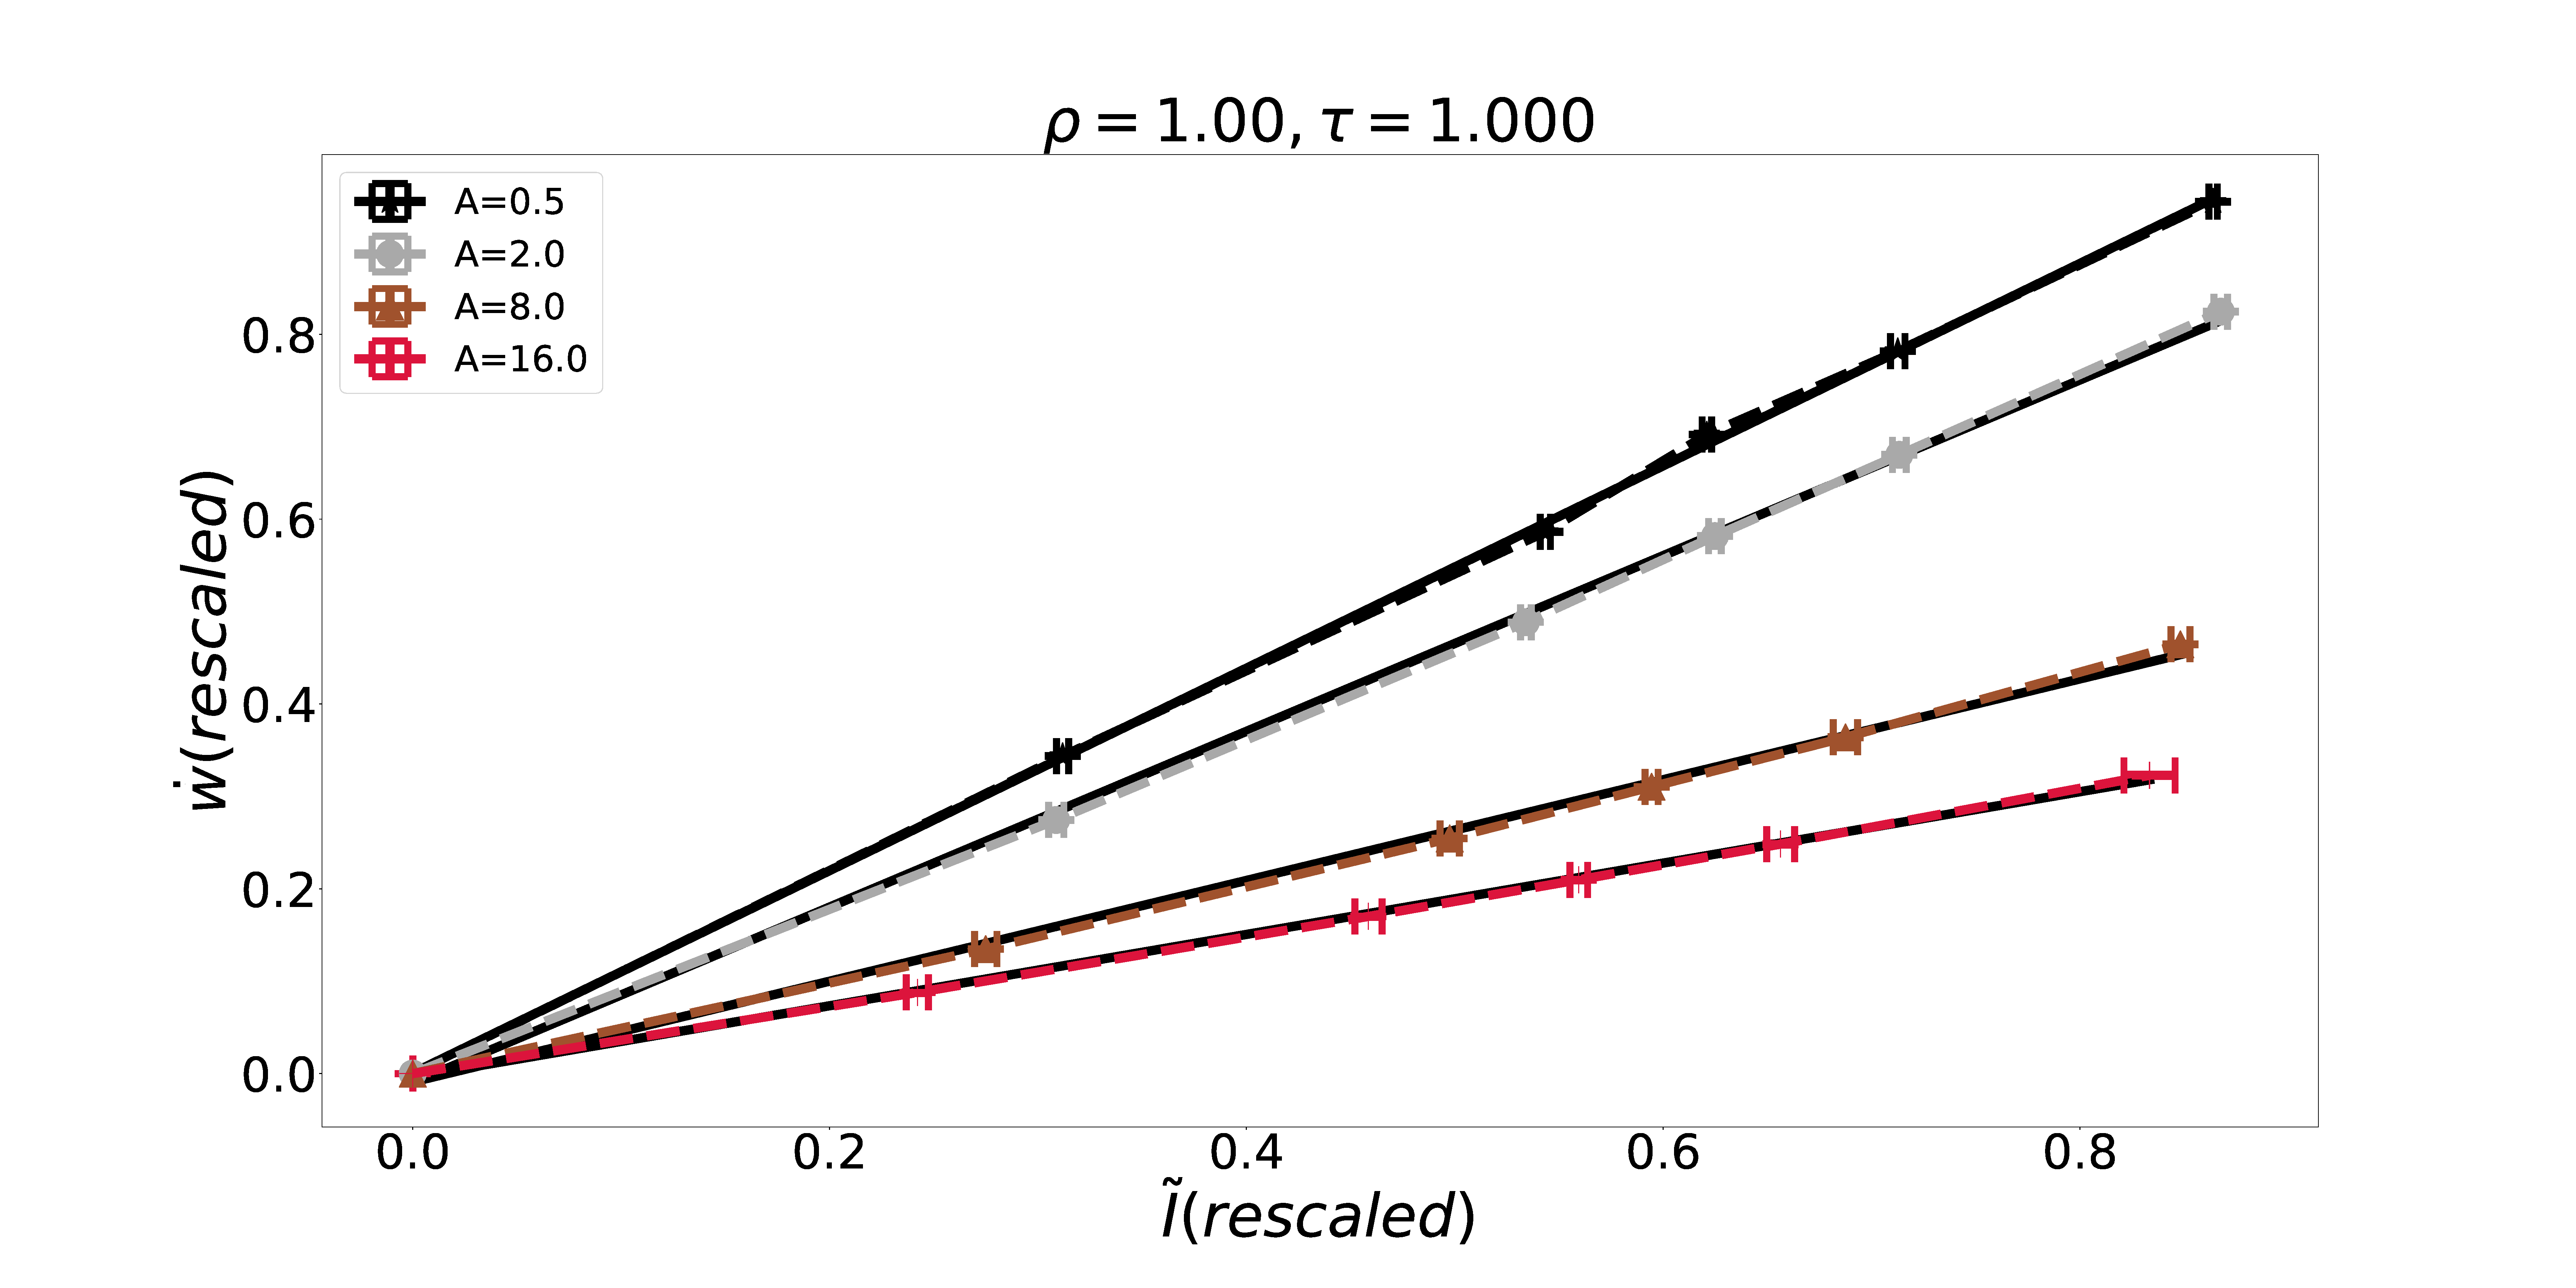
\includegraphics[scale=0.1, clip=True]{Plots_dW_tI_Suri_R1.00_A16.00_U1.000.pdf}
    \caption{}
    \label{Fig:n}
\end{figure}

\begin{figure}
    \centering
    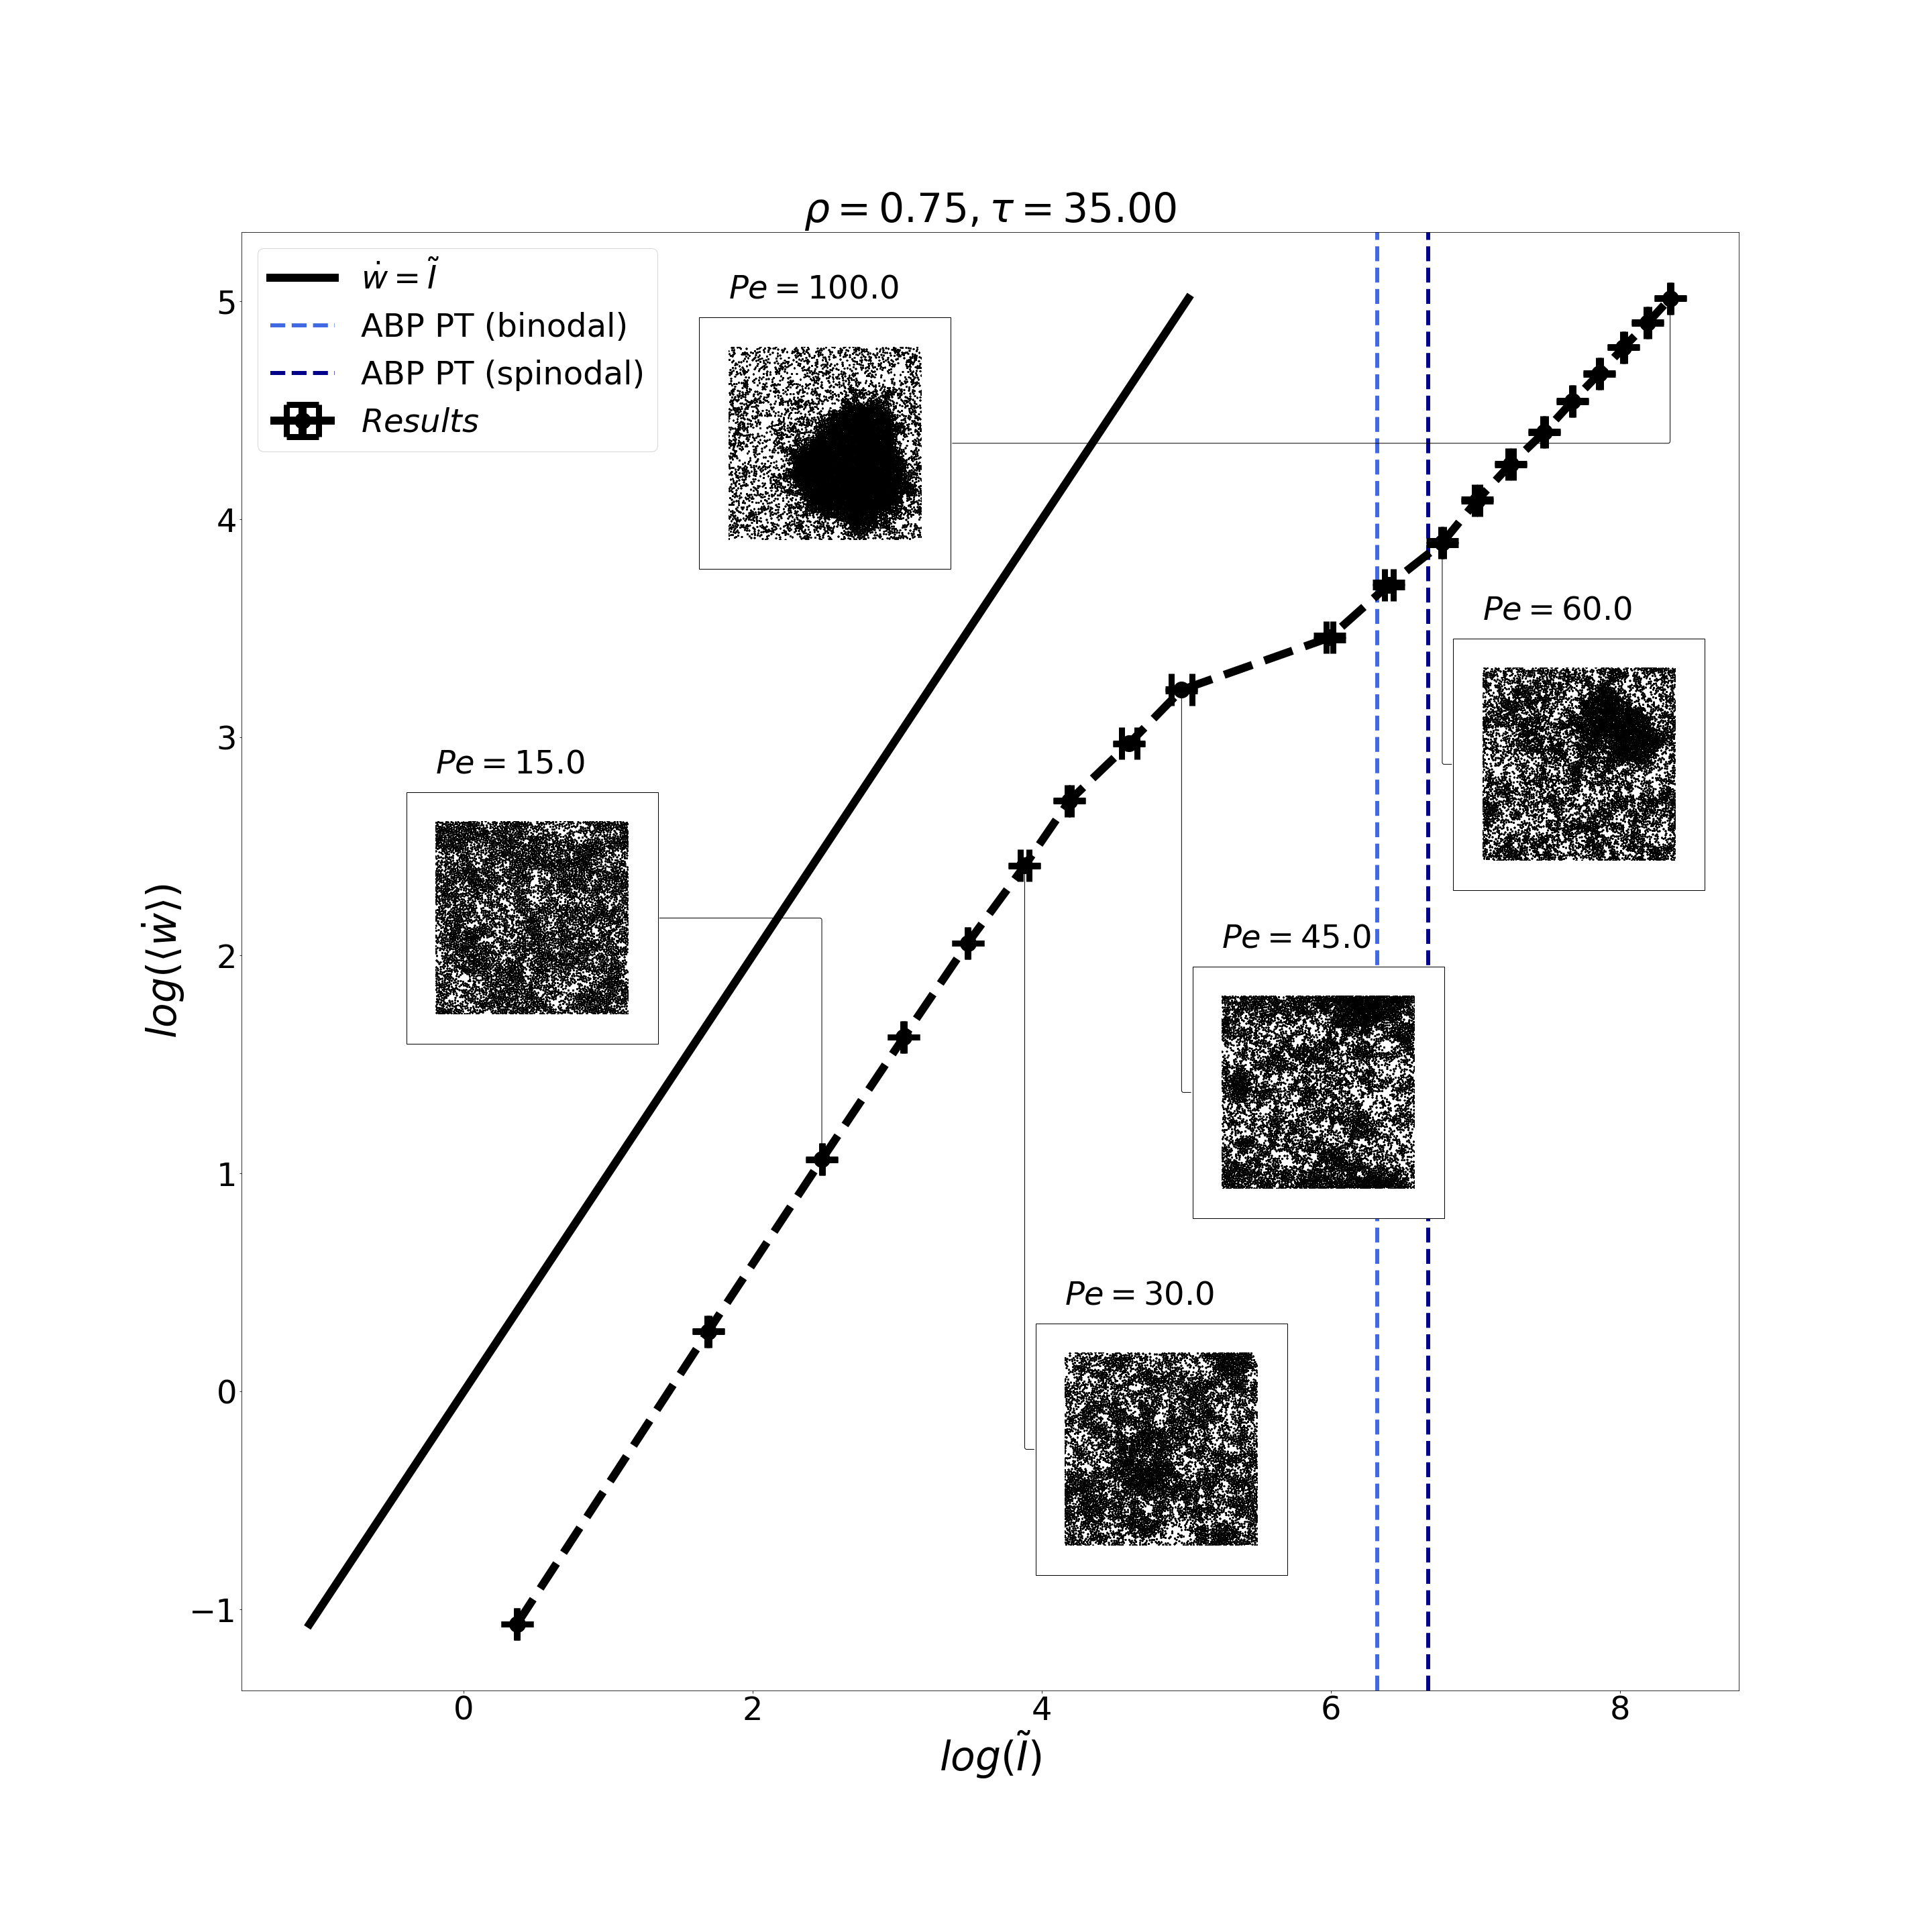
\includegraphics[scale=0.1, clip=True]{log_dW_tI_PT_R0.75_T35.00.png}
    \caption{}
    \label{Fig:n}
\end{figure}

%\begin{figure}
%    \centering
%    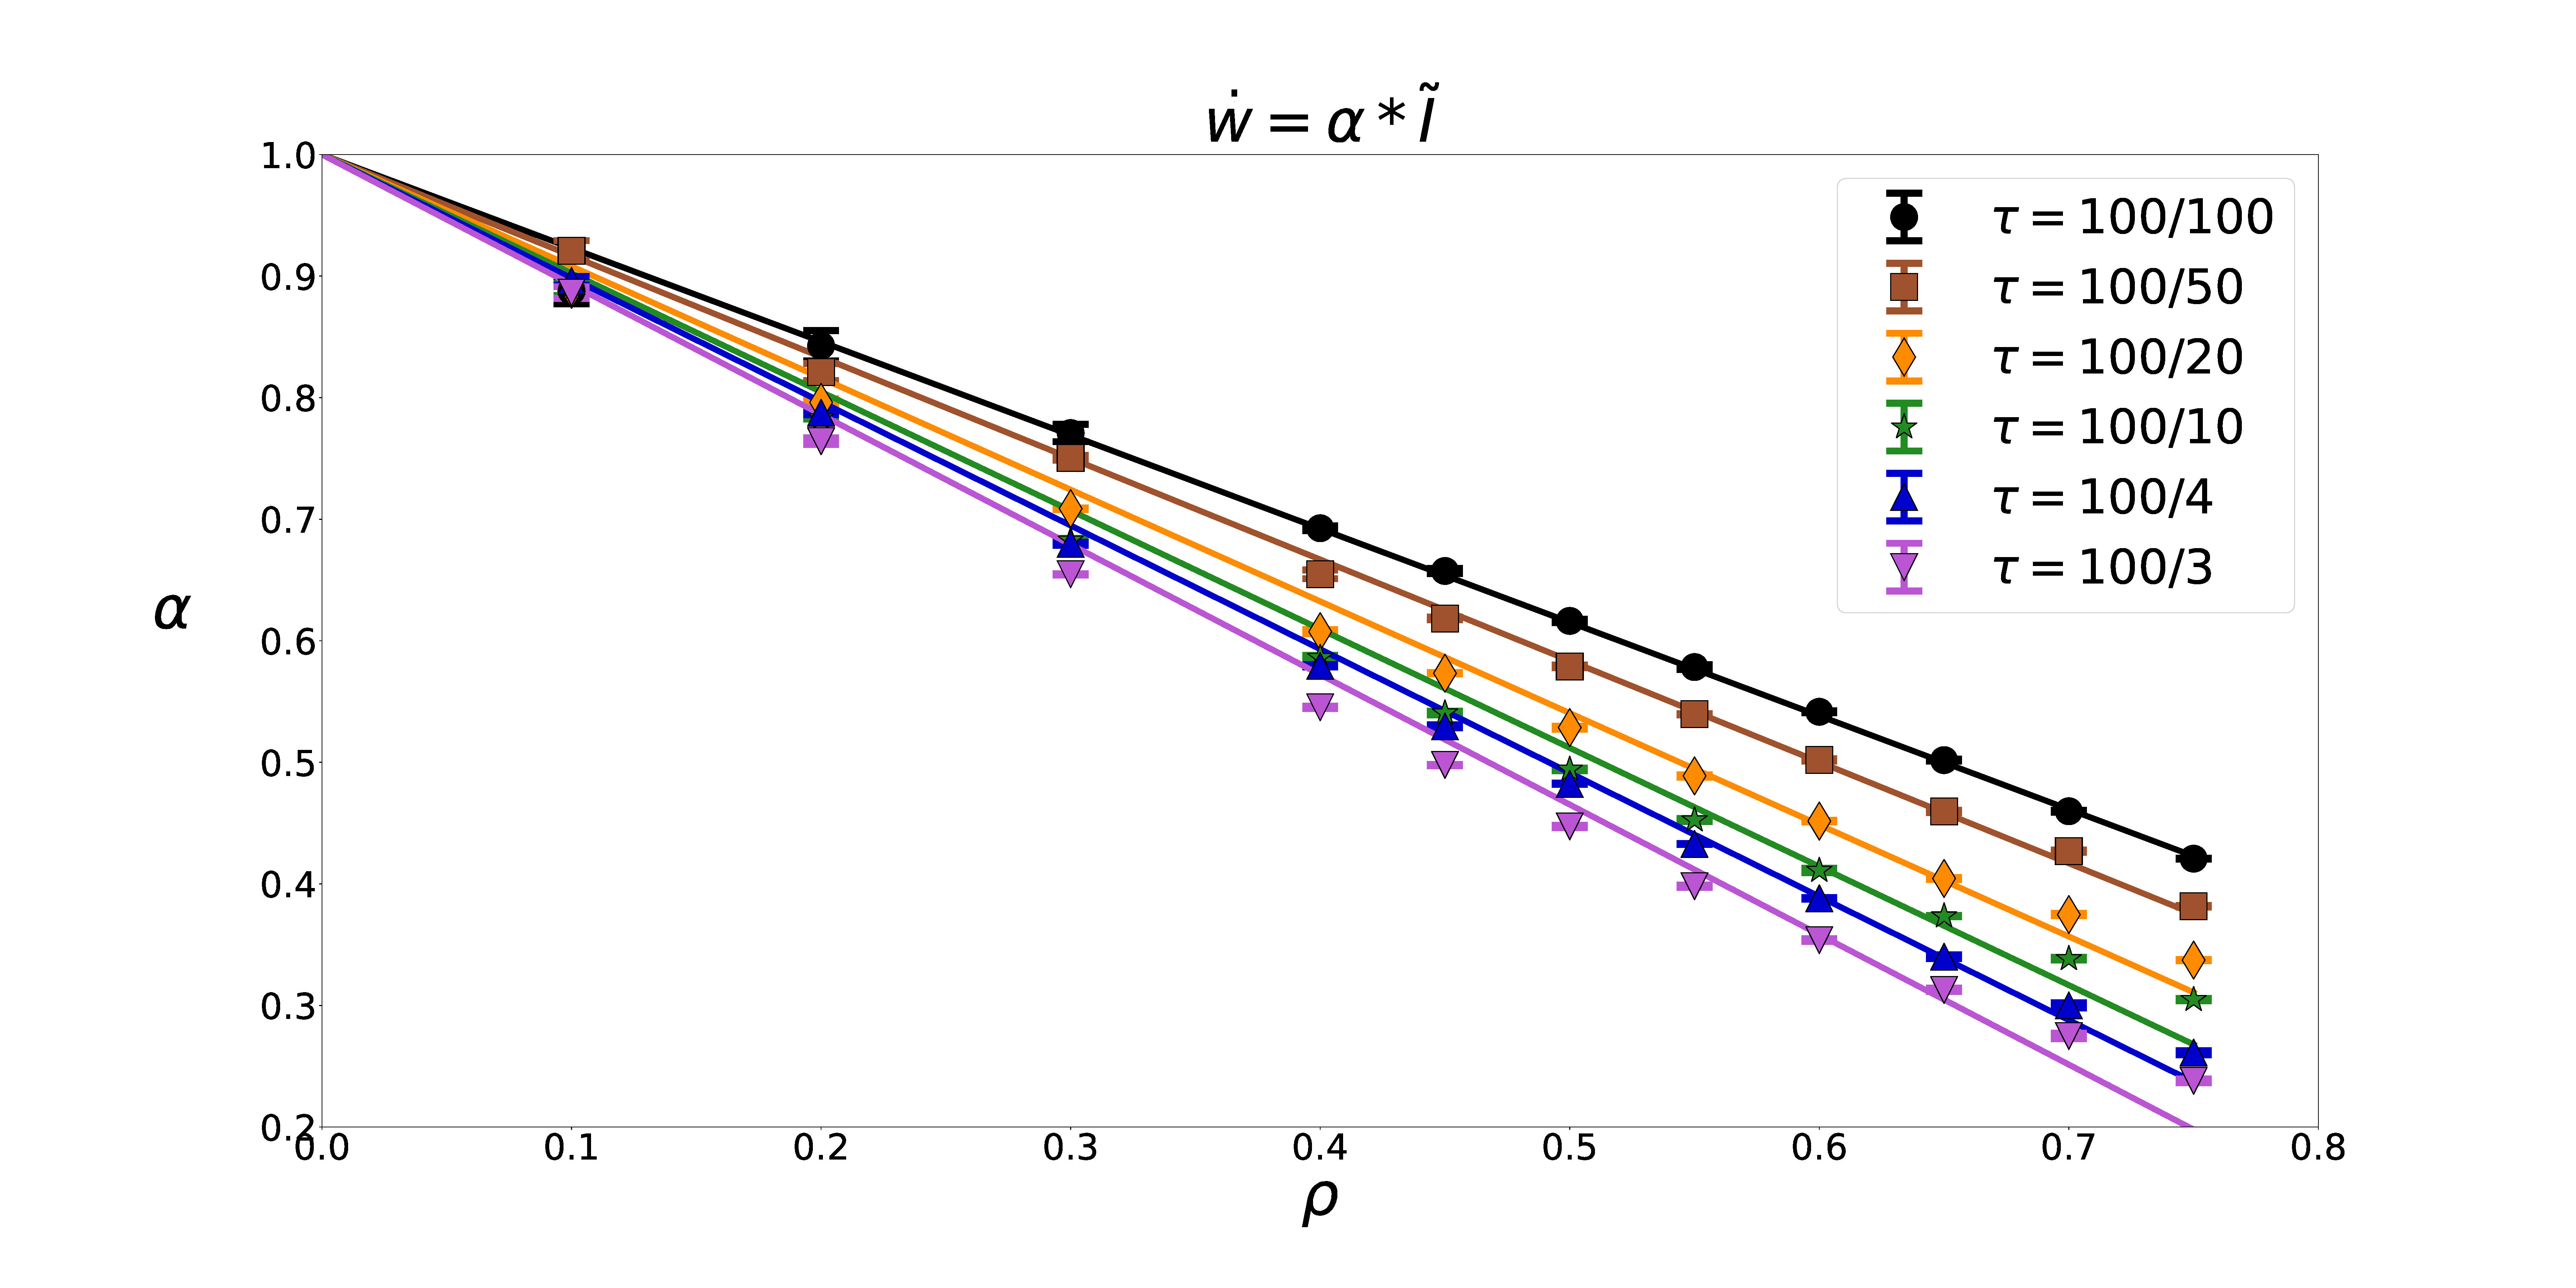
\includegraphics[scale=0.1, clip=True]{Results_xR_yA.pdf}
%    \caption{}
%    \label{Fig:n}
%\end{figure}

\begin{figure}
    \centering
    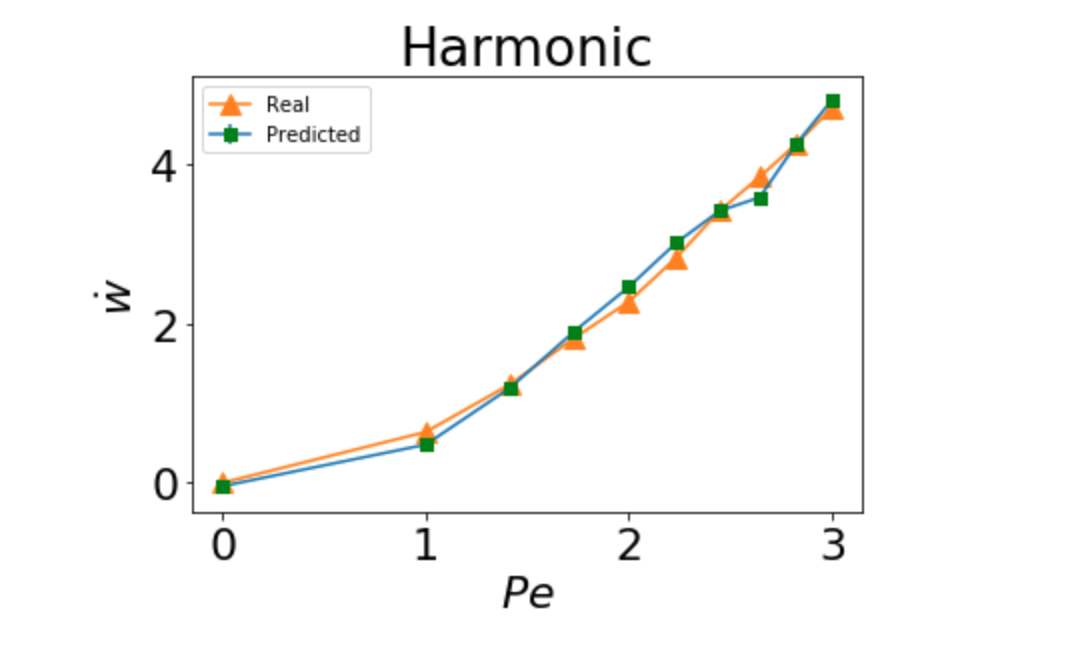
\includegraphics[scale=0.5, clip=True]{harmonic.png}
    \caption{}
    \label{Fig:n}
\end{figure}

\begin{figure}
    \centering
    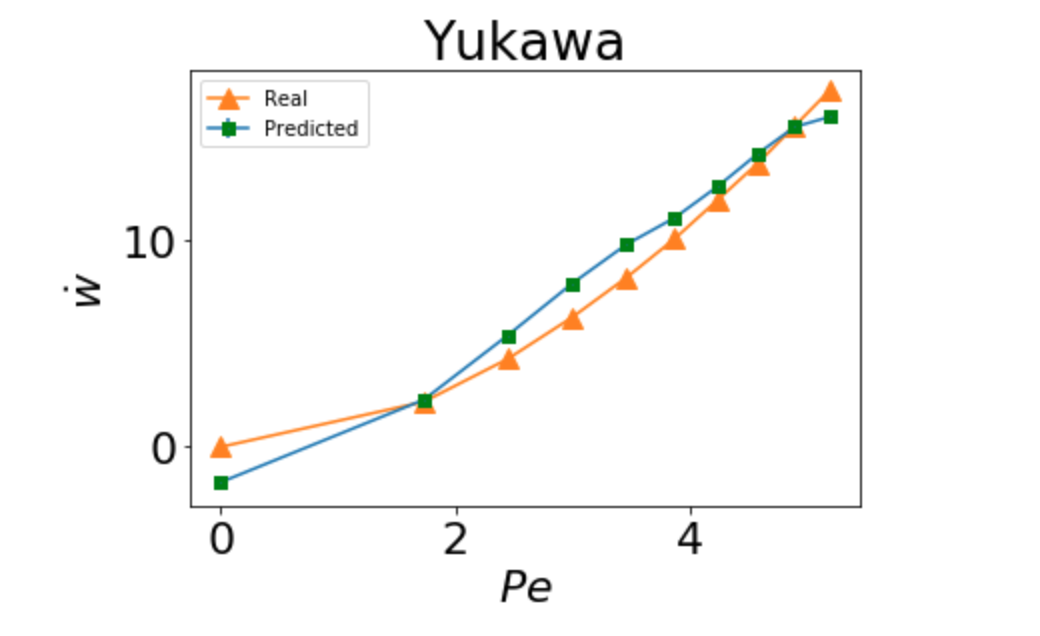
\includegraphics[scale=0.5, clip=True]{yukawa.png}
    \caption{}
    \label{Fig:n}
\end{figure}

\begin{figure}
    \centering
    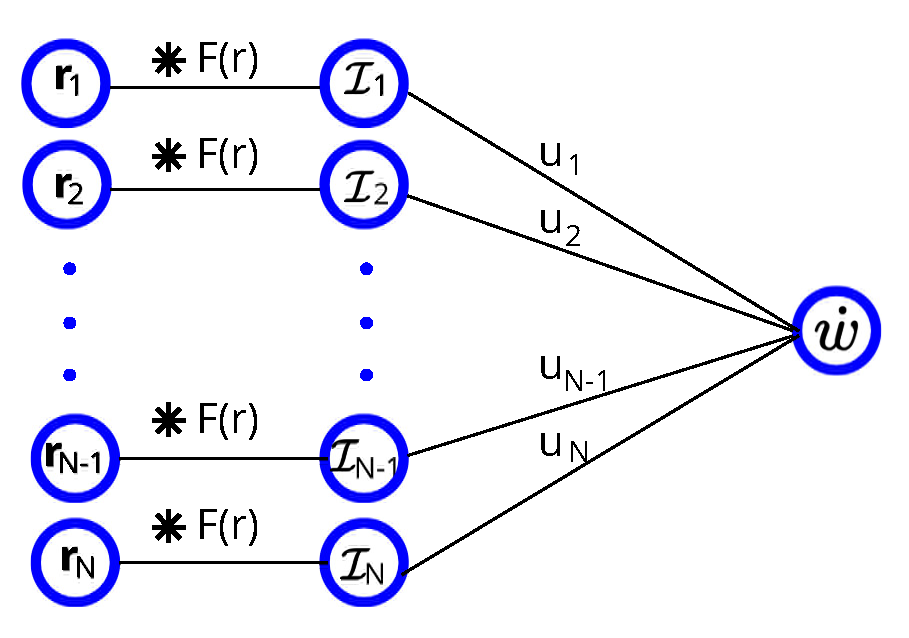
\includegraphics[scale=0.5, clip=True]{ML_architecture.pdf}
    \caption{The machine learning architecture consists of a convolutional layer, which performs the operation ${\bf r}_i * F(r) = \sum_{j \neq i} F(r_{ij})$, where $j$ runs over a set number of nearest neighbors. The function $F$ is expressed in a basis of Gaussian functions and the coefficients are learned by the machine. The second layer fully connects the convolutional layer neurons, labeled as $\mathcal{I}_i$, to the output neuron through the weights $u_i$ and a bias $b$:  $\sum_i u_i {\mathcal{I}_i} +b = \dot{w}$. The weights $u_i$ are constrained to be equal to ensure particle indistinguishibility.}
    \label{Fig:ML}
\end{figure}


\bibliography{References.bib}

\end{document}
